\documentclass[twocolumn, 10pt, a4paper]{memoir}
% standard packages
\usepackage{titlesec, blindtext, color}                                  % standard packages
\usepackage[usenames,dvipsnames,svgnames,table]{xcolor} % extra colors
\usepackage{graphicx}    
\usepackage{amsmath}                                                  % figures
%\usepackage{natbib}                                                          % bibliography
\usepackage[nosectionbib]{apacite}
\usepackage[hyphens]{url}
\usepackage{xcolor}
\usepackage[english]{babel}
\usepackage{multirow}                                              % correct hyphenation (afbreekstreepjes)
\usepackage{booktabs}                                                     % for midrule in tables
\usepackage{array}
\usepackage{float}
\newcolumntype{P}[1]{>{\raggedright\arraybackslash}p{#1}}
\usepackage[modulo, switch]{lineno}   % use for linenumbers at the sides
\usepackage{siunitx}
% PAGE MARGINS
\usepackage[top=2.5cm, bottom=2.5cm, left=2cm, right=2cm]{geometry}
\usepackage[export]{adjustbox}
\usepackage[font={small,it}]{caption}

% FONT
\usepackage[lf]{berenis}
\renewcommand*\familydefault{\sfdefault}
\usepackage[T1]{fontenc}
% for other fonts, and how to install them, see the LaTeX Font Catalogue:
% http://www.tug.dk/FontCatalogue/
\openany
% LINE SPACE
\linespread{1.2}                          % more space between lines
\setlength{\parindent}{7mm}       % indenting first line paragraph
\setlength{\columnsep}{7mm} % space between columns
\linenumbers
% TABLE OF CONTENTS
% for subsubsection headers (e.g. 2.1.3), write subsubsection
% for subsection headers (e.g. 2.1), write subsection
\setsecnumdepth{subsection}        % in text
\settocdepth{subsubsection}              % in table of contents
\renewcommand{\cftdot}{}          % for no dots in table of contents
\cleardoublepage

% HYPHENATION (afbreekstreepjes)
% set words that are not abbreviated correctly (expand list when necessary)
\hyphenation{catch-ment areas a-na-lyse}

\graphicspath{ {./images/} }
%%%%%%%%%%%%%%%%%%%%%%%%%%%%%%%%%
% headers: page numbers and running titles
%%%%%%%%%%%%%%%%%%%%%%%%%%%%%%%%%

\makepagestyle{ruled}
\makeevenfoot{ruled}{}{}{}  % empty footer
\makeoddfoot{ruled}{}{}{}   % empty footer

%% OLD HEADER LEFT PAGE
% header left page (text on left, middle and right slot empty)
%\makeevenhead{ruled}{\textcolor{gray}
%	{\makebox[6mm][l]{\thepage} $|$ \hspace{3mm} \leftmark}}{}{}
%%

% header left page (text on left, middle and right slot empty)
\makeevenhead{ruled}{}{}{\textcolor{gray}
	{ \leftmark \hspace{3mm} $|$ \makebox[6mm][l]{\thepage} }}
% header right page  (text on right, middle and left slot empty)
\makeoddhead{ruled}{}{}{\textcolor{gray}
	{\leftmark \hspace{3mm} $|$ \makebox[6mm][r]{\thepage}}}

% first page of chapter
\titleformat{\chapter}[hang]{\vspace{-34mm}\huge}{\thechapter\hspace{20pt}\textcolor{gray}{|}\hspace{20pt}}{0pt}{\huge}
\aliaspagestyle{chapter}{chapterheader} % for no page numbers on first chapter page


%%%%%%%%%%%%%%%%%%%%%%%%%%%%%%%%%
% for background figure first page
%%%%%%%%%%%%%%%%%%%%%%%%%%%%%%%%%

\usepackage{eso-pic}
\newcommand\BackgroundPic{%
	\put(-1,-1){%
		\parbox[b][\paperheight]{\paperwidth}{\vfill
			\raggedleft
			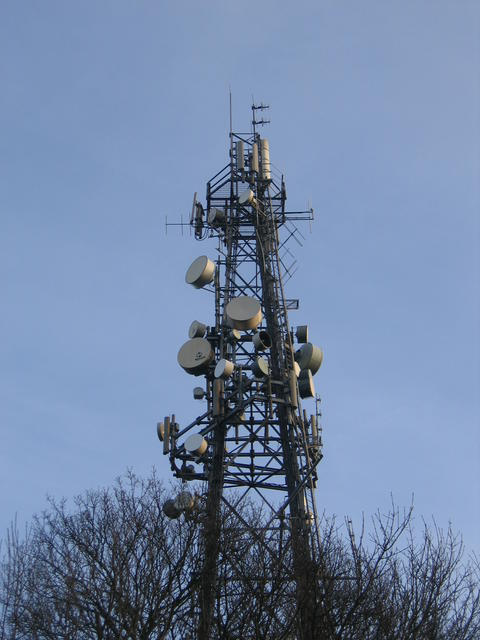
\includegraphics[width=\paperwidth,height=\paperheight]{CML_tower_bush}%
			\vfill
}}}



%%%%%%%%%%%%%%%%%%%%%%%%%%%%%%%%%
%%%%%%%%%%%%%%%%%%%%%%%%%%%%%%%%%
% START
%%%%%%%%%%%%%%%%%%%%%%%%%%%%%%%%%
%%%%%%%%%%%%%%%%%%%%%%%%%%%%%%%%%

\begin{document}
	
	\thispagestyle{empty}                    % otherwise it gives page number on first page
	\pagestyle{empty}
	\frontmatter
	\firmlists                                       % for less space between items in lists
	
	
	%%%%%%%%%%%%%%%%%%%%%%%%%%%%%%%%%
	% TITLE PAGE
	%%%%%%%%%%%%%%%%%%%%%%%%%%%%%%%%%
	
	%\AddToShipoutPicture*{\BackgroundPic} % for backgroundfigure
	
	\twocolumn[
	\begin{@twocolumnfalse}
		\begin{center}
			\vspace*{3cm}
			\color{white}
			\fontsize{20}{20} \textbf{Learning with links}\\
			\vspace{2cm}
			\fontsize{16}{16}\textbf{Estimating precipitation from Commercial Microwave Link signals using an all-encompassing neural network in the Netherlands}\\
			\vspace{12cm}
			\huge \textbf{Ludo Diender}\\
			\vspace{2cm}
			\large \textbf{Supervisors: Hidde Leijnse, Ruben Imhoff and Kirien Whan}\\
			\large \textbf{April 2022}\\
			\vspace{1cm}
			\large \textbf{MSc Thesis}
			\large \textbf{Hydrology and Quantitative Water Management Group}\\
			\large \textbf{Wageningen University}\\
		\end{center}
	\end{@twocolumnfalse}]
	
	
	%%%%%%%%%%%%%%%%%%%%%%%%%%%%%%%%%
	% ABSTRACT
	%%%%%%%%%%%%%%%%%%%%%%%%%%%%%%%%%
	
	\cleardoublepage
	
	\twocolumn [\begin{@twocolumnfalse}
		\chapter*{Abstract}\vspace{-6mm}       % the * prevents numbering of this section
		Having high-quality and high-resolution precipitation data is important for among others flood prediction. To gather this data on a country-wide level, the use of Commercial Microwave Links has been studied elaborately before. The best algebraic methods that are available to estimate precipitation via these links are based on a 4-step method. Previous research has shown it is possible and worthwhile to use neural networks on one of these steps at a time. This study aims to include all 4 steps in one all-encompassing neural network to create an easier and more comprehensible methodology.
		We made use of a Long Short Term Memory neural network to model the relation between the link signal and precipitation. A combination of automatic and manual calibration was carried out to study the sensitivity of the model to several hyperparameters and find the optimal combination. The final model is not able to capture the relationship. The difference in the observed and predicted precipitation range is large. Different preprocessing and scaling methods have been tested as well, to improve the predictions, with similar results. The impact of the different hyperparameters, both the automatically and manually calibrated ones, is shown to be negligible.
		Future studies should focus on using different (deep learning) models for the different steps of the algorithm and apply a more elaborate pre-processing to the data, as the neural network is not able to pick up on all the noise in the data. 
	\end{@twocolumnfalse}]
	
	%%%%%%%%%%%%%%%%%%%%%%%%%%%%%%%%%
	% TABLE OF CONTENTS
	%%%%%%%%%%%%%%%%%%%%%%%%%%%%%%%%%
	
	
	% to remove table of contents name and move the text up
	%\renewcommand{\contentsname}{\vspace{-3.5cm}}
	\twocolumn[\begin{@twocolumnfalse}
		\renewcommand{\contentsname}{\vspace{-3.5cm}}
		\chapter*{Contents}\vspace{-6mm}
		\tableofcontents*
	\end{@twocolumnfalse}]
	
	
	%%%%%%%%%%%%%%%%%%%%%%%%%%%%%%%%%
	% INTRODUCTION
	%%%%%%%%%%%%%%%%%%%%%%%%%%%%%%%%%
	
	% start on right side of page
	\cleardoublepage
	
	% start with page numbering 1, 2, 3 instead of i, ii, iii
	\pagestyle{ruled}
	\mainmatter          
	
	% Chapter name
	\chapter{Introduction}\vspace{-6mm}
	\section{Context and motivation}
	
	Having ample and correct precipitation data is important for a plethora of applications, including flood warnings, agriculture, river safety and shipping routes \shortcite{Chwala2019}. A high rain gauge density can help in providing this resolution \shortcite{Yoon2017}, but is not always availabe. Especially in data-scarce areas, where little precipitation is measured, Commercial Microwave Links (CML) have proven to be an excellent additional information source for precipitation data \shortcite{Overeem2021,Doumounia2014,Diba2021}. CML are back-haul links used by telecommunication companies to transfer information from one telecom station to the next using microwave signals (20-60 GHz). The links' signals get attenuated by rainfall by means of scattering and absorption (illustrated in Figure~\ref{fig: CML attenuation}). The received signal level is measured and stored by the telecommunication companies for monitoring purposes and can be used to retrieve path-averaged rainfall rates by calculating the attenuation. In the past 25 years, CML have been recognized as a valuable opportunistic method to estimate rainfall \shortcite{Leijnse2007, Ruf1996}. Recent research has been focussing on the use of CML data to measure rainfall in tropical regions, amongst others Sri Lanka \cite{Overeem2021} and Brazil \cite{RiosGaona2017a}. Although operational use of CML signal as precipitation data source is mainly limited by the availability and accessibility of the signal data, the technique has been widely researched.
	
	The first studies on the use of CML signals to retrieve rainfall rates were done by using a specific Power Law (PL)\footnote{See \citeA{Olsen1978} for more details} to relate the attenuation of the signal and the rainfall rate \shortcite{Overeem2011,Leijnse2007}. Several methods have been constructed based on this PL, including RAINLINK \shortcite{Overeem2011}. The RAINLINK methodology can be described with 4 steps: 
		\begin{enumerate}
			\item wet-dry classification
			\item baseline estimation
			\item wet antenna attenuation estimation
			\item rainfall rate retrieval
		\end{enumerate}
	This method has yielded good results in multiple studies \shortcite<e.g.>{deVos2019,Graf2020,Fencl2017}. Recently, the community has been exploring a more data-driven approach in the form of neural networks of different architectures. Neural networks are a subpart of Machine Learning that is inspired by the neural structure of the brain. A neural network consists of different layers of nodes (neurons) that are connected to each other. If the network contains more than one layer, it is considered a deep network and Deep Learning is used as equivalent naming. A neural network is able to learn the relationship between the input and output, without intervention from the modeller. Studies have been performed in Sweden, Israel \shortcite{Habi2019}, Germany \shortcite{Polz2020}, South Korea and Ethiopia \cite{Diba2021} on the use of such data-driven networks in relating CML signals to rainfall rates. Most of these use RAINLINK or a similar method as a benchmark. Previous studies have shown that data-driven models can be more accurate, less time-demanding and more robust in estimating rainfall rates compared to the PL method \shortcite{Polz2020,Pudashine2020}.  Neural networks are not a novelty in predicting rainfall \shortcite{French1992}, but the application to CML data has recently gained popularity.
	
	\begin{figure}[t]
		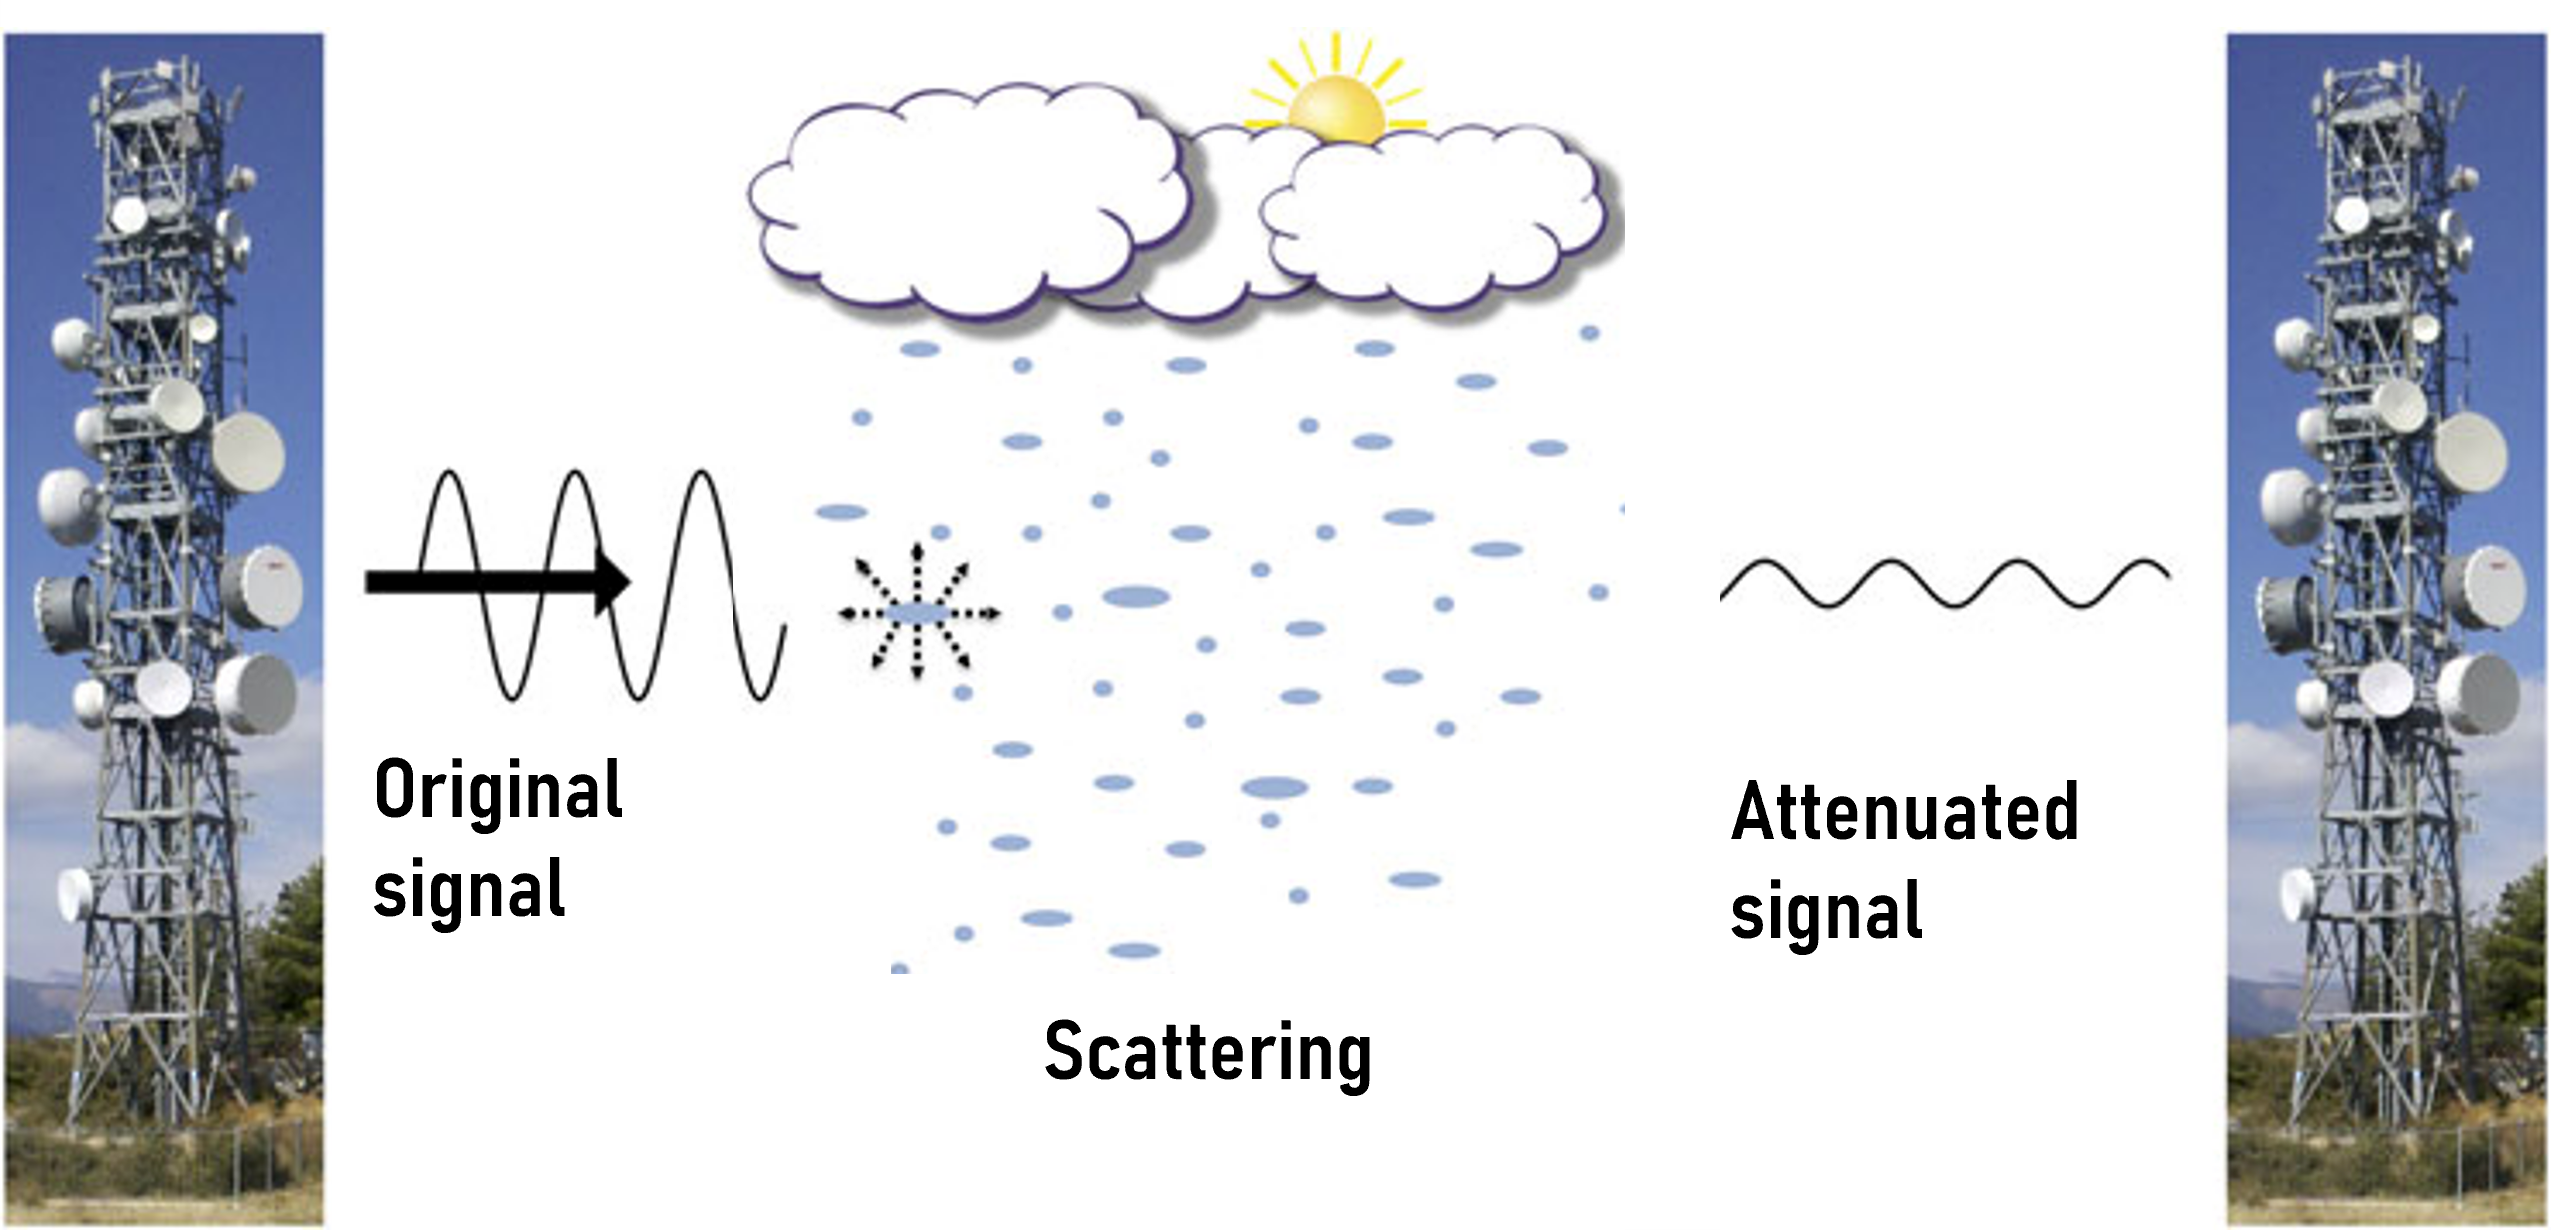
\includegraphics[width=8cm]{CML_concept_adapted}
		\caption{Concept of retrieving precipitation rates using CMLs. Adapted from \protect\citeA{Chwala2019} }
		\label{fig: CML attenuation}
	\end{figure}
	
	The few studies that have been performed on the combination of neural networks and CML, all focussed on a specific part of the RAINLINK methodology. \citeA{Polz2020} and \shortciteA{HabiYear} put emphasis on the wet-dry classification. \citeA{Pudashine2020} based their work around rainfall rate retrieval and \citeA{Habi2019} constructed a combined model with both aspects present, where he uses a separate Machine Learning model per aspect. All of these studies use a certain amount of preprocessing and error filtering, aside from the deep learning, to deal with the other aspects of the original PL algorithm.
	
	In focusing on a specific part of this method, the models can get more and more elaborate and complicated. Neural networks or deep learning can be a very versatile and powerful tool, but they come at the expense of understandability. The models can be tuned very specifically to the goal of the study \shortcite<e.g.>{Habi2019}, but it takes more and more time to understand why the model produces a certain output. Deep learning should in theory be able to deal with all steps of the algorithm. Having specific models for every step allows for a more specific but more complex models. An overarching, less complex and inclusive effort to model all steps of the RAINLINK algorithm at once has not been performed yet. This study aims to make use of the power of neural networks to deal with all steps in the RAINLINK algorithm at once. A deep learning effort to take all these steps into account has not yet been performed. 
	
	
	\section{Research questions}
	This study focuses on two main research questions.\newline
	1) How does a Neural Network perform on estimating rainfall rates from Dutch Commercial Microwave Link data by replacing all steps at once of the RAINLINK algorithm?
	2) What model (hyper)parameters have the largest influence on this performance?
	By answering these questions, this study will give a first impression of the power of neural networks to deal with raw data in combination with Commercial Microwave Links.
	
	\section{Thesis contents}
	This thesis starts with a description of the data that is used (Section~\ref{ch: field}). In Section~\ref{ch: methods}, the methodology of this study is described. This includes an explanation on Neural Networks, data preprocessing and the set-up of this model study. Afterwards, in Section~\ref{ch: results} the results are presented and interpreted. These results and the approach used in this study are discussed in Section~\ref{ch: discussion}, which is followed by the conclusion in Section~\ref{ch: conclusion}.
	
	
	
	
	
	
	%%%%%%%%%%%%
	% FIELD SITE AND DATA
	%%%%%%%%%%%%
	 
	\cleardoublepage
	\chapter{Data}\vspace{-6mm}\label{ch: field}
	In this study, two types of data are used: Commercial Microwave Link (CML) signal data which is used as input to the model, and precipitation observations (gauge-adjusted radar) as reference to train and evaluate the model. Both types of data will be elaborated upon in this section.
	
	
	\section{Commercial Microwave Link} \label{sec: CML data}
	The CML data used in this research is the same as used in previous research \shortcite{Overeem2016}.
	The CML data is retrieved from NOKIA microwave links, operated by T-Mobile. The dataset spans from January 14 2011 until June 30 2013. The dataset consists of  3101 links, but as shown before by \shortciteA{Overeem2016}, not all of these links are useful or continuously available. The total number of links used will therefore be lower, depending on the availability of the data. On average, around 2500 links are used at a time. The minimum and maximum Received Signal Level (RSL) in decibel-milliwatts (dBm) is stored at 15-minute intervals. The power resolution of this data is 1 dB. 
	
	\begin{figure}[h]
		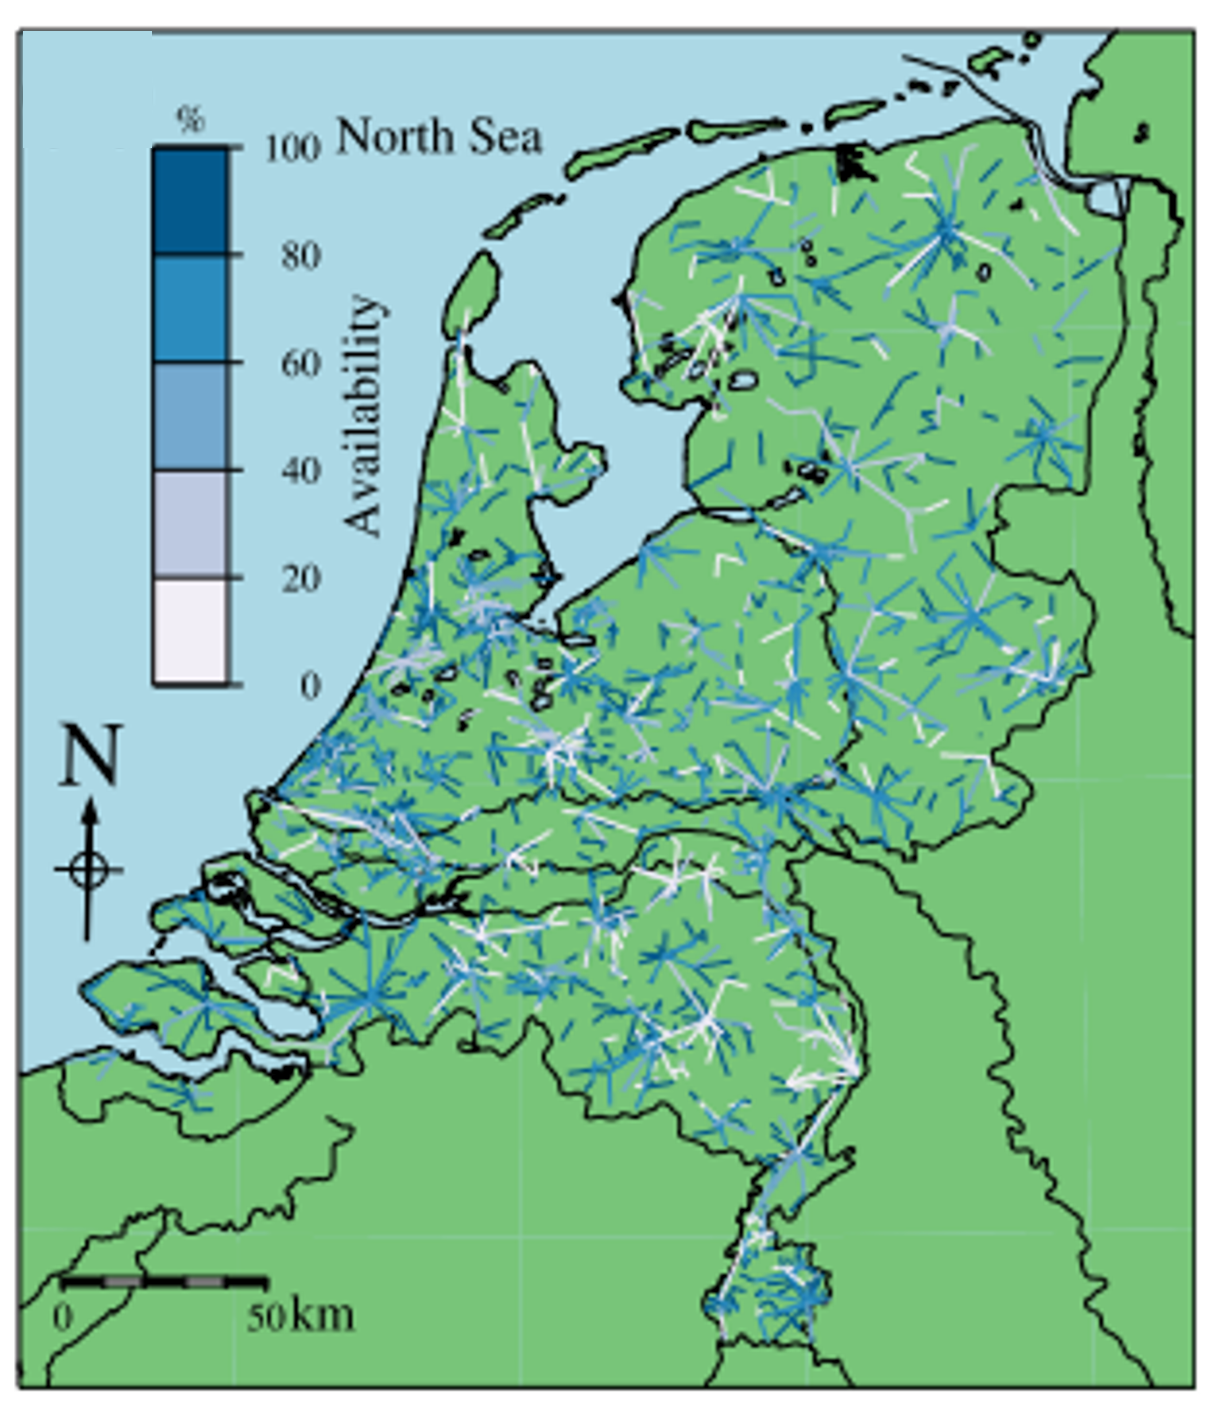
\includegraphics[height= 9cm]{Dutch_CML_network}
		\caption{Used CML network in the Netherlands. Retrieved from \protect\citeA{Overeem2016}}
		\label{fig: cmlnetworkmaps}	
	\end{figure}


	\begin{figure}[t]
		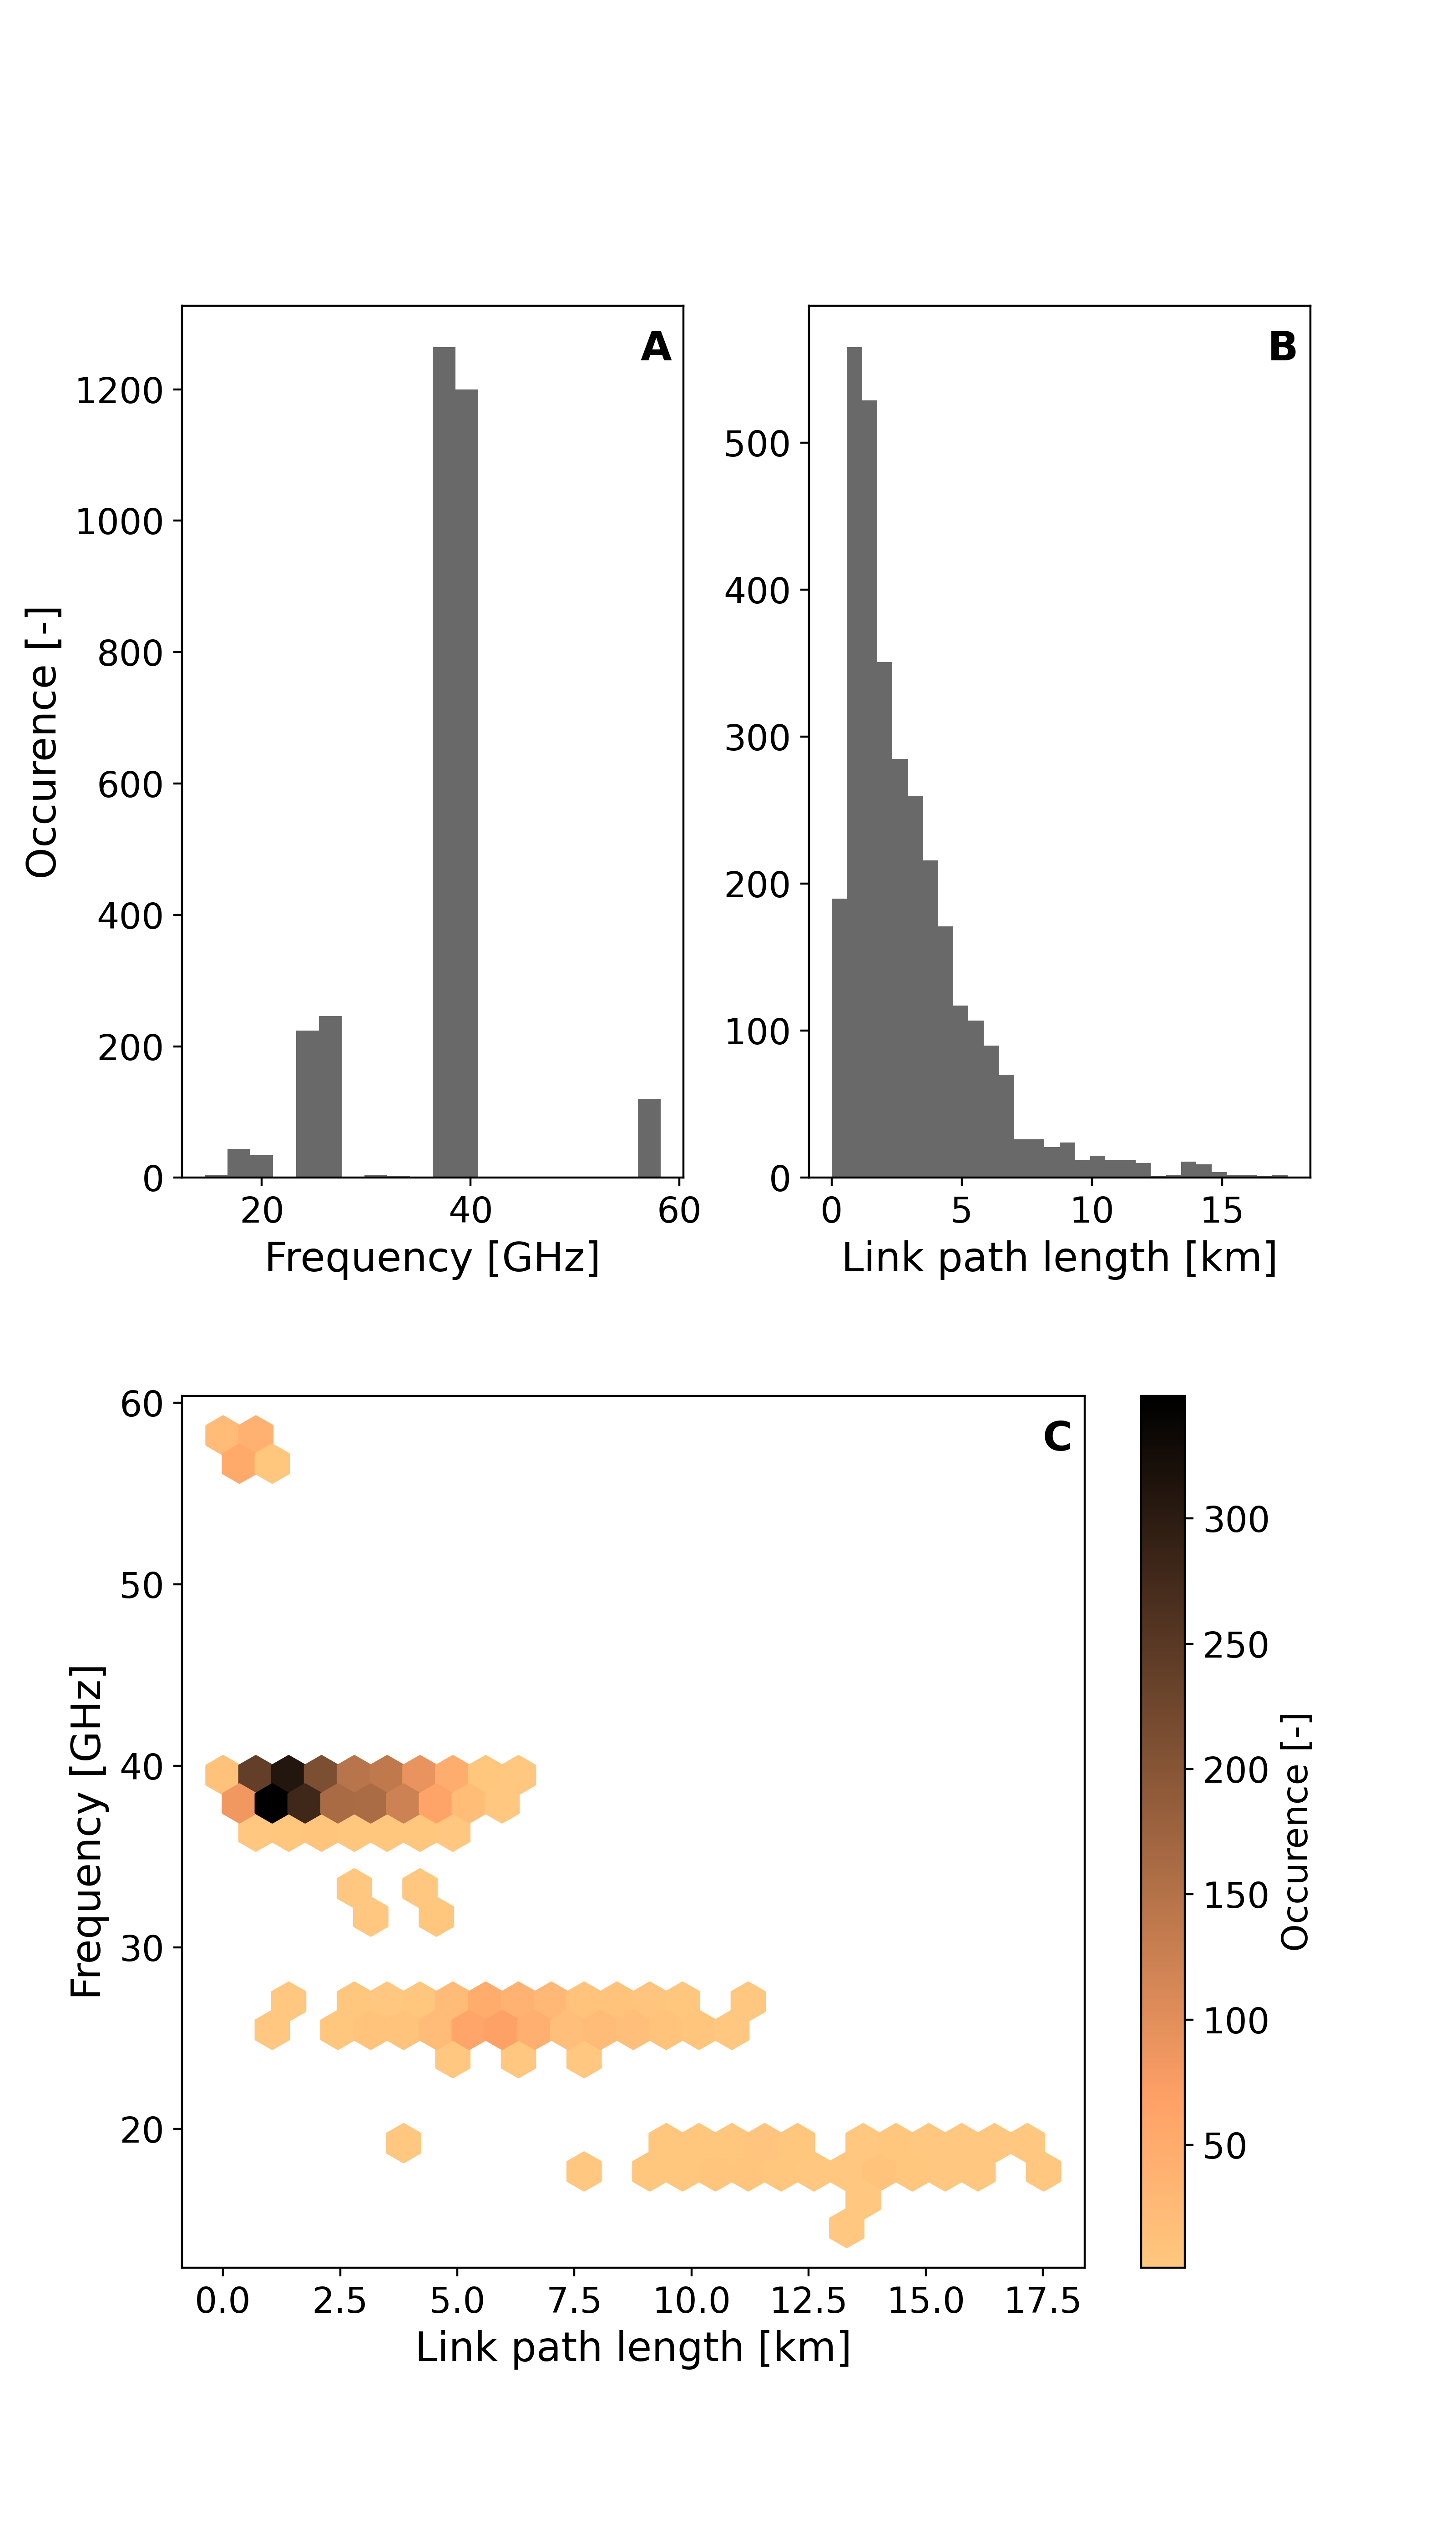
\includegraphics[width=10cm]{val_freq_dist}
		\vspace*{-1cm}
		\caption{Overview of the frequency distribution and link path length for the links in Figure~\ref{fig: cmlnetworkmaps}, with a) the frequency distribution, b) the link path length distribution and c) the occurence of the combination of the two parameters. Figures apply to the final independent test set covering half of 2013 (see Section~\ref{sec: method datasplitting})}
		\label{fig: CML validation}
	\end{figure}

	Apart from the dynamic time signal data, static metadata is included as well. This includes coordinates of the start and end point of the link, distance between these points and frequency per link. Figure \ref{fig: cmlnetworkmaps} shows the distribution of the links throughout the Netherlands, where the highest link density can be found around urban areas. The frequency at which the links operate and the distance the links cover, determine the attenuation for the links' signal caused by precipitation. They also influence, among others, the baseline of the signal, which is the second step in the RAINLINK methodology. Their respective distributions can be found in Figure~\ref{fig: CML validation}a and b. Figure~\ref{fig: CML validation}c shows the combined distribution of the distance and frequency. The spikes in the frequency distributions indicate that the links roughly operate at 4 different frequencies. The distance distributions shows that although most links operate at quite short distances (<4 km), there are still links included in the data set that cover over 5 or even 10 km. The effects of link path length and frequency on the estimation of precipitation has been discussed before by \citeA{Leijnse2008}.
		
	\subsubsection*{Practical data limitations}
	The CML dataset previously described is an enormous dataset. A single dataset contains around 80 million datapoints. Due to lack of computational resources, an underperforming High Performance Cluster at Wageningen University and various technical errors that we had absolutely no influence on, a depricated dataset has been used for the final modelling effort. This includes only 10 links per dataset (see Section~\ref{sec: datapreprocess}. The links were chosen based on their overall data availability.
	
	\section{Gauge-adjusted radar precipitation} \label{sec: Ref prec data}
	The precipitation observations in this study are from the gauge-adjusted radar rainfall product\footnote{Freely available as "Radar precipitation climatology" via http://climate4impact.eu} from KNMI with a resolution of 1 km\textsuperscript{2}. The radar measurements are adjusted (calibrated and validated) with the use of both automated and manual rain gauge networks operated by the Royal Netherlands Meteorological Institute (KNMI). The gauge-adjusted radar observations are available at a 5-min temporal resolution. To match the 15-min intervals from the CML data, the precipitation data is summed to 15-min intervals. This dataset is of high quality, fully available in the considered time period (Jan 2011 - June 2013) and can be considered the reference precipitation product for the Netherlands. Other studies that used the same gauge-adjusted radar data in combination with CMLs include \shortciteA{Overeem2016} and \shortciteA{Imhoff2020}.

	
	%%%%%%
	% METHODS
	%%%%%%
	
	\chapter{Methods} \label{ch: methods}
	This chapter describes the methodology of this study. The chapter starts with a general explanation on neural networks and their functioning to get acquainted with terms and parameters in Section \ref{sec: NN explain}. Section~\ref{sec: datapreprocess} deals with the preprocessing of the input data to the model and subsequently model selection is described in Section~\ref{sec: modelselection}. Which model runs are performed and how their results are evaluated will be treated in Section~\ref{sec: EvalStats}.
	\section{Neural network explanation} \label{sec: NN explain}
	\subsection{Goal and concepts of neural networks} \label{sec: NNConcepts}
	Neural networks are a subset of models within the Machine Learning (ML) environment. All models within the ML space are data-driven, i.e. without pre-specified relationships between input and output. These data-driven models aim to figure out this relationship via self-learning techniques.
	The biggest advantages of such models are that 1) they are very versatile: they can adapt to various circumstances and can be used in a wide range of applications, and 2) they can learn relationships that we do not have a physical explanation for yet. Through multiple iterations, the models can improve by minimizing or maximizing a loss function. The loss function can be interpreted as a score for the model: the worse the score, the more the model needs to adjust itself (see Section~\ref{sec: Learning NN}).It improves by optimizing parameters of simple weighted sums in the model. Similar to physically-based and conceptual models, it is up to the modeler to determine when the model performs well enough. The self-learning ML models will stop learning after a certain criterion is met, or when a specified number of iterations has passed.
	
	Neural networks are inspired by the structure of the human brain with neurons and synapses, hence the name neural network. The network consists of one or multiple layers of nodes that are connected with each other. When the network has more than one layer, it is called a deep neural network and it is referred to as Deep Learning. Every single connection between nodes (or between nodes and input/output) is represented by a weight and a bias. These weights and biases are the bread and butter of neural networks. They determine the underlying relationships between different parts of the input signal, the connections within the model and the relation to the final output. Training a neural network is all about adjusting the weights and biases in such a way that the desired output is created. At every node, a weighted sum is calculated based on these weights and biases and it is passed to an activation function. This activation function yields one value, which will be passed to the following nodes in the model.
	Because of the very general structure of neural networks, they form a very versatile set of models. Research efforts in neural networks span from image classification and speech recognition to time series prediction and weather forecasts.
	
	\subsection{Neural network architectures} \label{sec: NN architecture}
	The versatility of neural networks allows for a wide range of different model architectures to choose from. Every architecture has its own strengths and weaknesses. For image recognition for example, the most common type of neural network is a convolutional neural network (CNN). In time series prediction, the most common architecture is the recurrent neural network (RNN), which is therefore most suited for precipitation estimation using Commercial Microwave Links.
	
	RNNs are looping-based architectures, which make them ideal for dealing with sequences. The core unit of RNNs, the Recurrent Unit (the blue blocks in Figure \ref{fig: multilayer RNN}), is used multiple times. The output of the unit is added to the input of the next step in the same recurrent unit. This creates an architecture that is well suited for time series with sequential data patterns. How many layers of these recurrent units are used in a model depends on the modeler and can be tuned (see Section \ref{sec: modelselection})
	
	One of the limitations of default RNNs is the lack of memory in the model. Information from the start of a sequence is quickly lost throughout the model. A Long Short Term Memory (LSTM) model circumvents this problem by having an extra stream of information. This stream of information carries aspects of the previous time steps and can be viewed as a 'memory highway'. Every layer of the network has a separate memory stream which carries information from the start of the sequence. At every LSTM cell, information is taken from the memory state as input to the cell, and an adapted memory state is given as output. Most cells in an LSTM model have three input streams: the memory state, the new input and the hidden output state from the previous time step. Within each cell, the three input streams are used to produce three output states as well: the updated memory state, a hidden output for the next cell in the sequence and a hidden output for the next layer in the model. The conversion from these three inputs to three outputs is where the weights and biases come into play in an LSTM model. As an LSTM cell is a recurrent cell as well, there is one cell with weights and biases per layer of the network. Information is recurrently added to this cell. A schematic representation of the model used in this study can be found in figure~\ref{fig: multilayer RNN}.
	
	After the information has passed through all LSTM layers of the model, the final hidden outputs are fed into the fully connected or dense layer (see figure~\ref{fig: multilayer RNN}). This layer takes the intermediate output from the LSTM cells and connects them to the desired output of the model. The dense layers outputs a sequence of values, the same length as the input sequence. In this study, a many-to-one architecture is used. This means that a sequence of signal levels is used to predict one rainfall rate at a specific time step. Referring to figure~\ref{fig: multilayer RNN}, only the rightmost output ($O_n$) is considered the output of this model.
	
	For more information on the internal functioning of LSTM cells, a more in depth explanation of their power and the evolution to their current shape and form, the reader is referred to \citeA{Staudemeyer2019}.
	The LSTM approach in this study is similar, although not identical, to \citeA{Habi2019} and \citeA{Pudashine2020}. 
	
	\begin{figure*}
		\center
		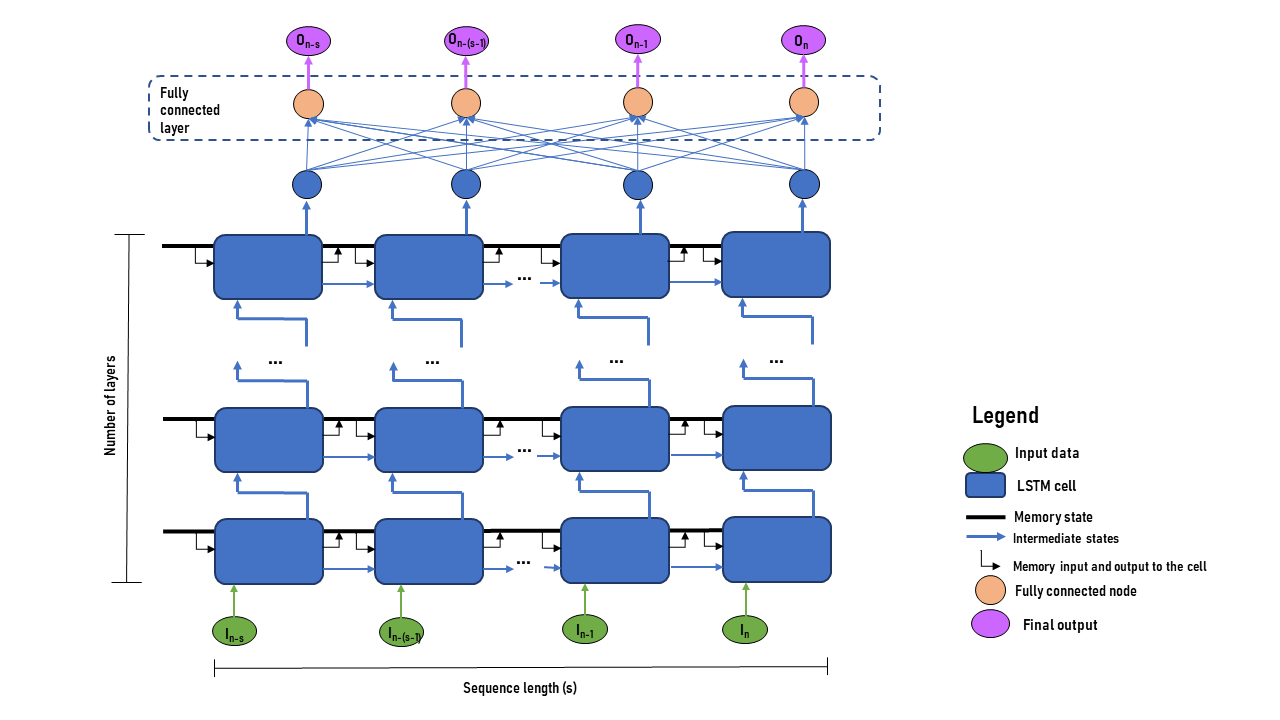
\includegraphics[width=\textwidth]{C:/Users/ludod/Documents/GitHub/Thesis_HWM2021/Thesis/images/Schematic_LSTM_TR_23_3_LudoDiender.png}
		\caption{\textit{Schematic representation of the LSTM model. Data is fed upwards through the model, where the top rightmost output is the final output of the model in a many-to-one architecture. The size of the intermediate states is given by the hidden size (Table~\ref{tab: hyperparamtable}) }}
		\label{fig: multilayer RNN}
	\end{figure*}
	
	\subsection{Learning process of neural networks} \label{sec: Learning NN}
	The self-learning ability of neural networks is mainly relying on the loss function. The model calculates the error between its output and the target output and tries to adjust accordingly. The selected loss function determines among others the behavior of the model. In this study, a standard Mean Square Error (MSE) loss function is used as a basis:
	\begin{equation} \label{eq: MSE}
		MSE = \frac{1}{n} \sum_{i=1}^{n} (y_i - \hat{y_i})^2,
	\end{equation}
	where ${y_i}$ is the predicted 15-min interval precipitation, $\hat{y}$ is the observed 15-min interval precipitation and $n$ is the number of samples.
	MSE as a loss function has been used before in similar studies \cite{Pudashine2020, Diba2021}. These studies, however, had a more elaborate preprocessing of the data to correct for the inherently skewed nature of precipitation distributions. \citeA{Habi2019} showed that the loss function can also be altered to correct for this skewness by using a Rain Distribution Factor (RDF). In this research, the application of an RDF serves two purposes:
	
	\begin{itemize}
		\item Penalize negative predictions to force the model into predictions bigger than or equal to zero. A random initialization can cause negative output which is physically impossible and should be avoided.
		\item Penalize the model more for higher target variables. This steers the model towards a better prediction of the actual precipitation events instead of focusing on the dry samples.
	\end{itemize}
	\vspace{3mm}
	The RDF is defined as:
	\begin{equation}
		\label{eq: RDF}
		RDF_i =\begin{cases}
			3, & y_i < 0\\
			1-c_s e^{c_r\cdot{}\hat{y}}, & \text{otherwise},
		\end{cases}
	\end{equation}
	where $y_i$ is the predicted rainfall rate, $\hat{y}$ is the observed rainfall rate and $c_s$ and $c_r$ are hyperparameters, set to $0.95$ and $-5$ respectively in accordance with \citeA{Habi2019}.
	
	The combination of Eq~\ref{eq: MSE} and Eq~\ref{eq: RDF} leads to the final loss function used in this thesis (Eq~\ref{eq: final_loss})
	
	\begin{equation}
		\label{eq: final_loss}
		Loss_i = \frac{1}{n} \sum_{i=1}^{n} RDF \ (y_i - \hat{y_i})^2
	\end{equation}
	
	To update and improve the model prediction, an optimizer (or propagation algorithm) is selected. Such an optimizer is a mathematical set of differential equations that determines how the model learns. In this study, the Adaptive Moment (ADAM) optimizer will be used. ADAM is one of the more recently introduced optimizers and has been shown to outperform other optimizations methods \cite{Kingma2014}. In simple terms: the method is looking for an optimum (minimum or maximum) per weight. Based on this gradient, the weight is adjusted up or down to minimize the loss function. As calculating the full gradient field for all weights present in the model is a tedious task, ADAM is a stochastic method, that takes a randomly selected subset of the data and uses that to calculate the gradients. This might lead to more steps, but the steps are less computationally intensive and typically lead to an improved performance.  
	The ADAM optimizer is back-propagated. This implies that the final layer of the network is updated first and the learning process works itself back to the start of the model. In this study, the fully connected layer at the end of the LSTM is updated first before the model improves and adjusts the LSTM cells itself. A back-propagated model is chosen in this study since it is the most common type of neural network, easy to implement, fast, flexible and generally well performing \cite{Staudemeyer2019}.
	
	The speed at which the model learns is determined by the learning rate. If set incorrectly (i.e. too high), the model can overfit, meaning that the weights and biases are well chosen for the trainingset but perform poorly on the validation and test set. 
	
	\subsection{Available hyperparameters} \label{sec: Avail hyper}
	The versatility of neural networks is generally perceived as one of the biggest advantages of these type of models. However, it does leave the modeller with a lot of options to choose from in creating a neural network for their specific task. The parameters that refer to the architecture and set-up of the neural network are called hyperparameters. Table~\ref{tab: hyperparamtable} highlights the available hyperparameters in this model. The hyperparameters will, for the purpose of this thesis, be divided in three groups: Structure, Data and Effiency. Structure hyperparameters relate to the structure of the model: how is it designed and how often will it run. Data parameters are related to the input data into the model; they are determined by the type of data and the goal of the study. The Efficiency group contains hyperparameters that relate to the time it takes the model to run. In this group, there is always a balance between performance and computational intensity. It should be noted that in the end, all hyperparameters influence the computational speed of the model in some way or another. The proposed grouping is not strict but rather serves the purpose of dealing with hyperparameters with a specific function in a structured way.
	
	\begin{table*}[ht]
		\caption{Available hyperparameters and their function}
		\hspace*{\fill}
		\label{tab: hyperparamtable}
		\centering
		\renewcommand{\arraystretch}{1.5}
		\begin{tabular}{P{0.8cm}P{2.0cm}P{12.8cm}}
			\hline
			Group&Hyperparameter&Description\\
			\hline
			\multirow{4}{*}[-35pt]{\rotatebox{90}{Structure}}&Hidden size&Size of the intermediate hidden output within each LSTM cell. Higher hidden size allows for more complex relations\\
			&Learning rate&A multiplication factor that influences the speed at which the weights in the model are updated with each step of the ADAM optimizer. A high learning rate makes the model learn faster, but also makes it more prone to overfitting.\\
			&Number of epochs&The number of iterations the model performs to reach the final prediction. More epochs improve the performance of the model but take sginificantly longer to run.\\
			&Number of layers&Total number of layers in the model. A higher number of layers creates a model that can better identify complex dependencies in the data.\\
			\midrule
			\multirow{2}{*}[-14pt]{\rotatebox{90}{Data}}&Sequence length&Length of datasample used to predict one target value. Default sequence length: 8\\
			&Loss function&Metric that is used to judge the model performance on. Can be tailored towards the goal of the model. Default: RDF MSE\\
			\midrule
			\multirow{4}{*}[-15pt]{\rotatebox{90}{Efficiency}}
			&Batch size&The size of each batch of data, i.e. the number of sequences, that is fed to the model. The larger the batch size, the faster the model will be able to learn, but the less possiblities it has to update its weights and biases. Default batch size: 32\\
			&Optimizer&The algorithm that is used to update the weights and biases of the model internally. Default optimizer: ADAM\\
			&Scheduler&The algorithm that is used to run multiple combinations of hyperparameters simultaneously and decides when early stopping of trials is necessary. Default scheduler: ASHA\\
			
			\bottomrule
			
		\end{tabular}
		\hspace*{\fill}
	\end{table*}
	
	The process of calibrating hyperparameters in order to find an optimal combination (if it exists) is refered to as tuning. Not all hyperparameters were automatically tuned. Only the Structure hyperparameters were tuned, as the other two hyperparameter groups need to be determined based on the input data and the available computational resources. More details on the automatically tuned Structure hyperparameters can be found in Section \ref{sec: RayTune}. The Data and Efficiency group of hyperparameters are set based on convenience and literature study and will be elaborated on in Section \ref{sec: Nonauto tuning}.
	
	
	\section{Data preprocessing} \label{sec: datapreprocess}
	\subsection{Connecting CML and reference data}
	To train the model, a feature set (received signal levels) and a target set (precipitation observations) is needed. For every separate CML link and every time step, the corresponding amount of precipitation has been determined. To obtain this value, the middle point of each link has been determined and connected to the corresponding radar cell. This midpoint method is commonly used in CML research \cite{Pudashine2020, Diba2021}. More elaborate methods have been used by \shortciteA{Leijnse2007} for example, where a weighted sum of all cells that the link passes through was created. The impact of this decision will be discussed further on in this thesis (see Section~\ref{sec: middle link}).
	\subsection{Error filtering}
	A large part of the RAINLINK algorithm consists of error filtering. Because the algorithm cannot distinguish a signal distortion by rain or by a bird, this filtering is necessary. The spirit of Deep Learning models is that these errors do not need to be filtered out manually. Similar to Habi et al., just the 'no data' values have been removed from the dataset. The model is expected to handle other noise in the data by learning the patterns and adjust accordingly.
	\subsection{Data splitting and scaling} \label{sec: method datasplitting}
	A Deep Learning model with a varying set of hyperparameters needs three independent datasets to run: a training set, a validation set and a test set. The training dataset is used to improve the models' weights and parameters by feeding it through the ADAM optimizer, in which the model is updated in a backwards propagating fashion. The validation set is subsequently used to independently judge the performance of the model. This set needs to be as independent as possible, to prevent overfitting of the model.
	As different models with different combinations of hyperparameters are tested, a third independent test dataset is needed to check how well the best model out of these different combinations performs.  
	
	In creating the three separate datasets, multiple approaches can be taken. The core of the split is based on the IID principle \cite<Independent and Identically Distributed;>{Hampel1998}:
	
	\begin{itemize}
		\item There is little to no information leaked from one set to the other (truly independent datasets)
		\item There is enough data in each of the sets to cover a wide range of events and situations (comparable datasets and thus assumed identically distributed)
	\end{itemize}
	IID data ideally does not have any internal dependencies in the data left that could complicate the model's ability to generalize. 
	
	The data for the Netherlands has been split in a 40/40/20 for training, validating and testing respectively. Previous studies use varying ratios to split the data, with the one common aspect being a smaller test set compared to the training and validating \cite{Polz2020,Diba2021,Pudashine2020}. This particular split has been chosen as a rough average of these varying ratios.
	The year 2011 is used for training, 2012 for testing and 2013 (up until July 21st) for validating. By taking full years for training and testing, all seasons are incorporated and the datasets are assumed to have similar distributions. Considerations on and implications of this split will be discussed later on in this thesis in section \ref{sec: discussion datasplitting}.
	
	All three datasets contain the 10 links with the highest availability for their respective time period (see Section~\ref{sec: CML data}). The impact of the use of this depricated dataset is discussed briefly in Section~\ref{ch: discussion}.
	
	Having large outliers and ranges in the input data can cause the ADAM algorithm to have exploding gradients. Therefore, a scaling has been applied to both the features and targets. 
	The targets (precipitation observations) have been scaled using an inverse hyperbolic sine transformation, which is a variant on the more common log transformation \cite{Kilmartin1972}. To deal with zero values, which are ominous in precipitation data, and to handle extreme values better, Burbidge \citeA{Burbidge1988} introduced the inverse hyperbolic sine transformation. This transformation is defined as in Eq~\ref{eq: logsine}.
	
	\begin{equation}
		\label{eq: logsine}
		y_t = \log(y_i + \sqrt{y_i^2 + 1})
	\end{equation}
	where $y_t$ is the transformed variable and $y_i$ is the raw variable.
	Afterwards, the logsine-transformed precipitation data were scaled with the minimum and maximum per dataset, to create a value between 0 and 1. As three separate datasets were used, this implies three slightly different scalings. As the goal is to minimize information leakage from one dataset to the next, separate scaling is applied, in order to not further violate the aforementioned IID assumption. Scaling the datasets in a different way per dataset is not necessarily preferred in machine learning, as the model cannot reliably learn the scaling in order  to predict the precipitation rates. The values that the datasets have been scaled with however, are quite similar. This implies that although a different scaling is applied, the scalings are assumed to be similar and have no significant effect on the final predictions of the model.
	
	The features (RSL) have been scaled differently. As the base level of each CML is dependent on the link specifics, the median of each link per dataset has been subtracted from the signal. \citeA{Polz2020} showed that this is the best performing scaling for the CML data. Subsequently, the data has been divided by the standard deviation per dataset to obtain values that are closer to each other. By subtracting the median of each link from the signal, a very crude form of baseline estimation has been applied (step 3 in the RAINLINK methodology). As data needs to be rescaled anyways in order to avoid exploding or vanishing gradients, this specific scaling has been included in the methodology of this study. Similar to the previously described precipitation data scaling, the separate scaling per dataset is not assumed to cause a significant effect on the final predictions. 
	
	
	
	\section{Model selection} \label{sec: modelselection}
	This section deals with selecting the right model structure for the study at hand. It is worth noting that there might be multiple combinations of hyperparameters that lead to the same results (a variant on the concept of equifinality). In section~\ref{sec: Equifinality} this concept will be elaborated on and the impact on the followed procedure will be discussed.
	
	\subsection{Automated hyperparameter tuning} \label{sec: RayTune}
	A full grid search on all hyperparameters available to find the best combination is computationally infeasible. Therefore, this study uses 25 random combinations of hyperparameters, all within a limited range of values. This number of combinations is chosen to have a trade-off between computational intensity and having ample combinations to ensure a decent search. All 25 combinations are full model runs that start learning from scratch. The combinations are drawn using a Monte Carlo method on a continuous uniform distribution. This does not guarantee 25 perfectly distributed runs, but the continuous uniform distribution allows the edges of the parameter ranges to be taken into account and evaluated as well. 
	
	Selecting the combinations is done using the RayTune package \cite{Liaw2018}, which is a tuning-specific Python package that interacts with PyTorch (used in this study) and other Deep Learning packages. This study uses the Async Successive Halving Algorithm Scheduler (ASHA) to effectively search the hyperparameter space. The ASHA Scheduler is able to effectively implement parallellized computing (to decrease runtime) and a hard early stopping mechanism to terminate runs if they are not amongst the best few models after a while \cite{Li2018}. The ASHA Scheduler is the most common scheduler available in RayTune and performs well in most cases when no specific instructions regarding hyperparameter tuning are needed. 
	 
	After tuning, one combination of hyperparameters yields the best results after training. This combination is used to calculate the model performance based on the final independent testset. The ranges for the calibrated hyperparameters can be found in Table~\ref{tab: raytunetable}
	
	\begin{table}
		\caption{Ranges for the automatically tuned hyperparameters using RayTune.}
		\label{tab: raytunetable}
		\centering
		\renewcommand{\arraystretch}{1.5}
		\begin{tabular}{P{3.5cm}P{3.2cm}}
			\hline
			$Hyperparameter$&$Range$\\
			\hline
			Hidden size&$[8,32,64,128,256]$\\
			Learning rate&$1.0\times 10^{-6} - 1.0\times 10^{-3}$\\
			Number of epochs&$10 - 50$\\
			Number of layers&$[2,4,8,16]$\\
			\hline
		\end{tabular}
	\end{table}
	
	\subsection{Non-automated hyperparameter tuning} \label{sec: Nonauto tuning}
	Hyperparameters that are related to the data rather than the model itself are not tuned automatically. Hyperparameters in the Data group are tuned, but in a slightly less rigid way, i.e. manually, as it is easier to deduct which values should perform well on the input data.
	
	The sequence length is partly determined by how long rainfall events typically last in the Netherlands and their autocorrelation. As a starting value, a sequence length of 8 (15-min) timesteps is used \cite{Beek2012}. This means that the past two hours are used to predict the rainfall rate at the current time step. A sequence length of one hour (4 timesteps) and three hours (12 timesteps) will be evaluated as well to inspect the impact of a different sequence length.
	
	The loss function has a direct relation to the distribution of the input data. The chosen loss function (Equation \ref{eq: final_loss}) should be able to deal with the skewness of the data. To check if this is the case and whether the extra effort of including a RDF is worth it, a normal MSE loss function (Equation \ref{eq: MSE}) will be tested as well.
	
	From the Efficiency group, the batch size is the most important hyperparameter to evaluate. \citeA{Kandel2020} described the effect of the batch size on the final performance of the model. The batch size and the learning rate are intimately linked: a smaller batch size requires a lower learning rate and vice versa. A batch size of 32 is used as standard, but the options of batch sizes of 64 and 128 are explored as well. A batch size of 32 has been shown to be a good default value \cite{Bengio2012}. Using a power of 2 as batch size is common to fully use GPU processing power.
	
	\section{Experimental setup and evaluation of results} \label{sec: EvalStats}
	For this study, different model runs are performed. In the first run, all automatically tuned hyperparameters mentioned in Section~\ref{sec: RayTune} are included. The 25 different randomly chosen model runs, as picked by the random selector in RayTune, are shown in Table~\ref{tab: hyperparameter combi}. 
	
	\sisetup{table-number-alignment=right,exponent-product=\cdot}
	\begin{table}[t]
		\caption{Different hyperparameter combinations used for the tuning experiment.}
		\hspace*{\fill}
		\centering
		\renewcommand{\arraystretch}{1.2}
		\begin{tabular}{P{0.2cm}P{1cm}P{2cm}P{1.4cm}P{1.2cm}}
			\toprule
			\multicolumn{1}{c}{ID} & Hidden size & Learning rate & Number of epochs & Number of layers \\ \midrule
			\multicolumn{1}{l|}{1} & $8$   & $3.58\cdot10^{-4}$  & $37$       & $8$                \\
			\multicolumn{1}{l|}{2} & $32$  & $4.67\cdot10^{-6}$  & $26$       & $8$                \\
			\multicolumn{1}{l|}{3} & $8$   & $1.74\cdot10^{-5}$  & $47$       & $2$               \\ 
			\multicolumn{1}{l|}{4} & $128$ & $1.54\cdot10^{-6}$  & $27$       & $2$                \\
			\multicolumn{1}{l|}{5} & $64$  & $7.16\cdot10^{-4}$  & $41$       & $8$               \\
			\multicolumn{1}{l|}{6} & $32$  & $2.39\cdot10^{-4}$  & $47$       & $8$                \\
			\multicolumn{1}{l|}{7} & $128$ & $3.67\cdot10^{-4}$  & $33$       & $16$              \\
			\multicolumn{1}{l|}{8} & $32$  & $4.06\cdot10^{-5}$  & $15$       & $4$                \\
			\multicolumn{1}{l|}{9} & $8$   & $3.78\cdot10^{-6}$  & $26$       & $2$                \\
			\multicolumn{1}{l|}{10}& $32$  & $1.17\cdot10^{-4}$  & $15$       & $4$                \\
			\multicolumn{1}{l|}{11}& $64$  & $4.29\cdot10^{-4}$  & $12$       & $16$                \\
			\multicolumn{1}{l|}{12}& $64$  & $4.99\cdot10^{-6}$  & $23$       & $16$                \\
			\multicolumn{1}{l|}{13}& $256$ & $5.24\cdot10^{-5}$  & $12$       & $8$                \\
			\multicolumn{1}{l|}{14}& $32$  & $1.18\cdot10^{-5}$  & $14$       & $4$                \\
			\multicolumn{1}{l|}{15}& $64$  & $2.52\cdot10^{-6}$  & $19$       & $8$                \\
			\multicolumn{1}{l|}{16}& $32$  & $5.51\cdot10^{-6}$  & $11$       & $2$                \\
			\multicolumn{1}{l|}{17}& $128$ & $2.79\cdot10^{-4}$  & $23$       & $16$                \\
			\multicolumn{1}{l|}{18}& $32$  & $4.78\cdot10^{-5}$  & $34$       & $16$                \\
			\multicolumn{1}{l|}{19}& $32$  & $3.21\cdot10^{-6}$  & $26$       & $16$      \\
			\multicolumn{1}{l|}{20}& $64$  & $1.51\cdot10^{-4}$  & $12$       & $8$                \\
			\multicolumn{1}{l|}{21}& $32$  & $2.29\cdot10^{-4}$  & $35$       & $2$                \\
			\multicolumn{1}{l|}{22}& $64$  & $1.99\cdot10^{-4}$  & $40$       & $8$                \\
			\multicolumn{1}{l|}{23}& $8$   & $1.52\cdot10^{-4}$  & $20$       & $2$                \\
			\multicolumn{1}{l|}{24}& $128$ & $6.30\cdot10^{-5}$  & $41$       & $8$                \\
			\multicolumn{1}{l|}{25}& $8$   & $5.73\cdot10^{-6}$  & $24$       & $2$                
		\end{tabular}
		 \label{tab: hyperparameter combi}
	\end{table}
	The model run with the best score on the independent test set will be used to test different non-automatically tuned hyperparameter settings. This results in three more combinations of model runs per hyperparameter, where the batch size, the loss function and the sequence length are evaluated respectively with their ranges as put in Section~\ref{sec: Nonauto tuning}.
	
	For the final model run, only timesteps that show precipitation are taken into account. This functions as a very crude wet-dry classification, the first step in the RAINLINK methodology. By running the model only on rain samples, we investigate the impact of using such a wet-dry classification, as multiple previous studies included a model part on this step \cite{Habi2019}. 
	
	All these runs are performed on the depricated datasets. This includes 300.000 samples for the training, validation and test set. In ideal circumstances, the test set would be smaller but since the model runs were performed on a subset of the data, similarly sized datasets were chosen. In the training procedure, the sequences are constructed to be 1) continuous and 2) from just one link. The model knows it is dealing with a different link, but the spatial information of this link is not used. Although the frequency and link path length have an influence on the signal, the crude baseline estimation and the learning capabilities of the deep learning model are expected to be able to deal with this influence. 

	The model results will be evaluated using the coefficient of determination (R$^{2}$, see Eq~\ref{eq: R2}), the Coefficient of Variation (CV, Eq~\ref{eq: CV}) and the Root Mean Square Error (RMSE, Eq~\ref{eq: RMSE}):
	\begin{equation} \label{eq: R2}
		R^2 = 1- \frac{\sum_{i=1}^{N} (\hat{y}_i - y_i)^2}{\sum_{i=1}^{N} (y_i - \bar{\hat{y_i}})^2},
	\end{equation}

	\begin{equation} \label{eq: CV}
		CV = \frac{\sigma}{\bar{y}},
	\end{equation}

	\begin{equation} \label{eq: RMSE}
		RMSE = \sqrt{\frac{1}{n} \sum_{i=1}^{n} (y_i - \hat{y_i})^2}.
	\end{equation}
	In these equations, $y_i$ is the predicted 15-min precipitation rate, $\hat{y_i}$ is the observed 15-min precipitation rate, $\sigma$ is the standard deviation of the predicted 15-min precipitation rate and $n$ is the number of samples.
	
	These statistical evaluation metrics will be able to tell something about the fit of the model prediction to the observed values. The selected metrics are based on similar studies that use these metrics to evaluate their model performance \shortcite{Overeem2011, Pudashine2020,Diba2021}.
	
	%%%%%%%%%%%%%%%%%
	%%%% RESULTS %%%%
	%%%%%%%%%%%%%%%%%
	
	\chapter{Results} \label{ch: results}
	\subsection*{Automated hyperparameter tuning}
	Figure~\ref{fig: loss epochs} shows the validation loss for the 25 different combinations of hyperparameters. Due to the random initialization of each model, the starting losses differ between the runs. About half of the combinations show a decreasing loss over the epochs, which indicates the self-learning capabilities of the neural network. Some models hardly improve over the epochs or even worsen. This particuliar behaviour could be caused by the overfitting of the model on the training dataset. The best model yields a loss (RDF MSE) of 0.346 on the validation dataset. This best run corresponds to model ID 9 and the combination of hyperparameters can be found in Table~\ref{tab: hyperparameter combi}. The final loss on the test dataset is 0.204. This is lower than the error on the validation dataset. As both datasets are independent, this is not uncommon. It shows that the either the model is unexpectedly well fit for the test dataset, or the test dataset is an easier dataset to estimate precipitation rates for. This could be due to less errors or a more clear pattern in the signal-precipitation relationship.
	
	\begin{figure}[h]
		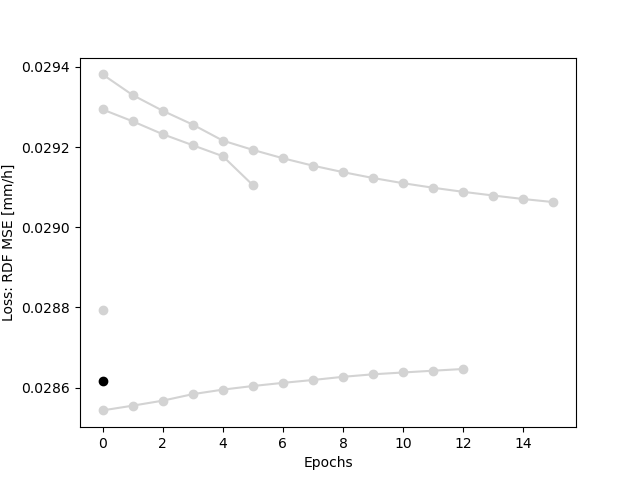
\includegraphics[width=\columnwidth]{ex_loss_epochs}
		\caption{The validation loss (RDF MSE) per epoch for all 25 tuning runs. The best model that will be used for subsequent model runs is depicted in black, all other runs are depicted in grey.}
		\label{fig: loss epochs}
	\end{figure}

	The performance of the best combination of hyperparameters on the final independent test set is depicted in figure~\ref{fig: scatter statistics}. This shows that the model, although it improved over time, manages to predict a small range of values the majority of the time. The observed range in precipitation rates and the modelled range in precipitation rates are vastly different, as the predicted values are only in a small range of -0.5-2.5 mm/h, while the observed rainfall rates are distributed on a significantly larger range of 0-22 mm/h. The CV of [INSERT CV] and RMSE of 0.413 do not tell the complete story of the prediction, as their values are in line with previous research \cite<0.83 and 0.64 respectively;>{Pudashine2020}. The R\textsuperscript{2} of 0.157 however does indicate the poorness of the modelled fit. The investigated hyperparameters for these runs are not the deciding factors in this modelling effort as the predictions and observations are still widely different. 
	\begin{figure}[t]
		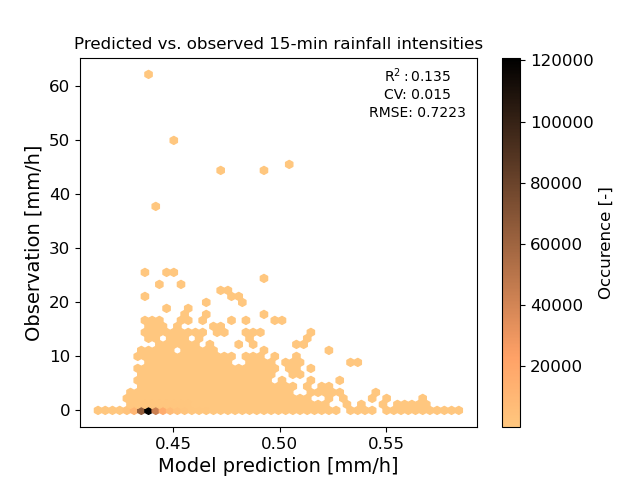
\includegraphics[width=\columnwidth]{scatter_final}
		\caption{Predicted versus observed precipitation for the best model configuration out of Figure~\ref{fig: loss epochs}.}
		\label{fig: scatter statistics}
	\end{figure}
	The model prefers to predict a value of around 0.2 mm/h for the cases in which no rain was observed. Due to the skewness of the dataset, there are more dry samples than wet samples. The chosen loss function (RDF MSE) was picked to accomodate for this skewness and focus more on the wet samples, but the results in Figure~\ref{fig: scatter statistics} indicate that it has not dealt fully with this skewness yet. The model also predicts negative precipitation rates, which are not realistic. Although the RDF has been altered to penalize negative predictions even more, the model has not learned to fully steer towards positive predictions. This mismatch in predicted and observed precipitation is possibly caused by both the skewness of the input (with which the model is not able to deal well) and the incorrect estimation of the baseline of the signal. Estimating the baseline of the signal too low could cause negative predictions for the precipitation rate. The impact of the skewness is shown in Figure~\ref{fig: onlyrain scatter} and a possible solution to the incorrectly baseline estimation is discussed in Section~\ref{sec: baseline}.
	
	
	\begin{figure}[H]
		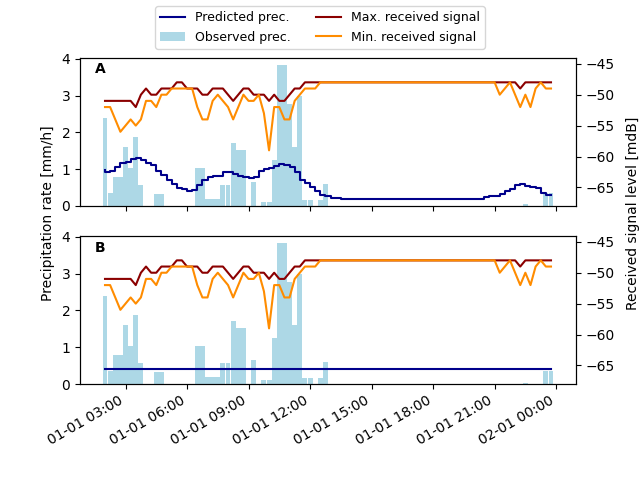
\includegraphics[width=\columnwidth]{CML_timesignal_faulty}
		\caption{The predicted precipitation rate for one precipitation event in 2013. Plot A depicts the predicted results using hyperparameter configuration 9 (loss: 0.347), plot B depicts the predicted results using hyperparameter configuration 7 (loss: 0.355). The configurations can be found in Table~\ref{tab: hyperparameter combi}. The colored lines indicate the CML signal and are the input data to the model. The black line is the final precipitation rate output.}
		\label{fig: CML timesignal}
	\end{figure}
	Figure~\ref{fig: CML timesignal} shows the prediction of the model for two different hyperparameter configurations for January 1\textsuperscript{st} 2013. Although the R\textsuperscript{2} reported in Figure~\ref{fig: scatter statistics} does not indicate a decent fit, the model is able to pick up some of the information present in the input signal in Figure~\ref{fig: CML timesignal}a. The precipitation rates are underestimated at almost all times and the baseline of the prediction is around 0.14 mm/h. The timing of the precipitation, especially the tail at the end of each event, is in most cases prolonged and smoothened out. This could be due to the wet antenna attenuation, which is not accounted for in this modelling approach. The lower subplot Figure~\ref{fig: CML timesignal}b shows a different hyperparameter configuration. The reported losses on the validation dataset for the two datasets are close to each other: 0.347 and 0.355 for configuration 9 and 7 respectively. This figure shows that a small difference in loss function can have a large difference in the predictive powers of the model, as configuration 7 predicts just one value around 0.4 mm/h. Based on this figure, one could argue that the chosen RDF MSE loss function is not suitable for the job, as different configurations with similar losses results in completely different predictions. Figure~\ref{fig: seqlen} shows the impact of picking a different loss function to possibly solve this issue.
			
	\begin{figure*}[t]
		\hspace*{-3cm}
		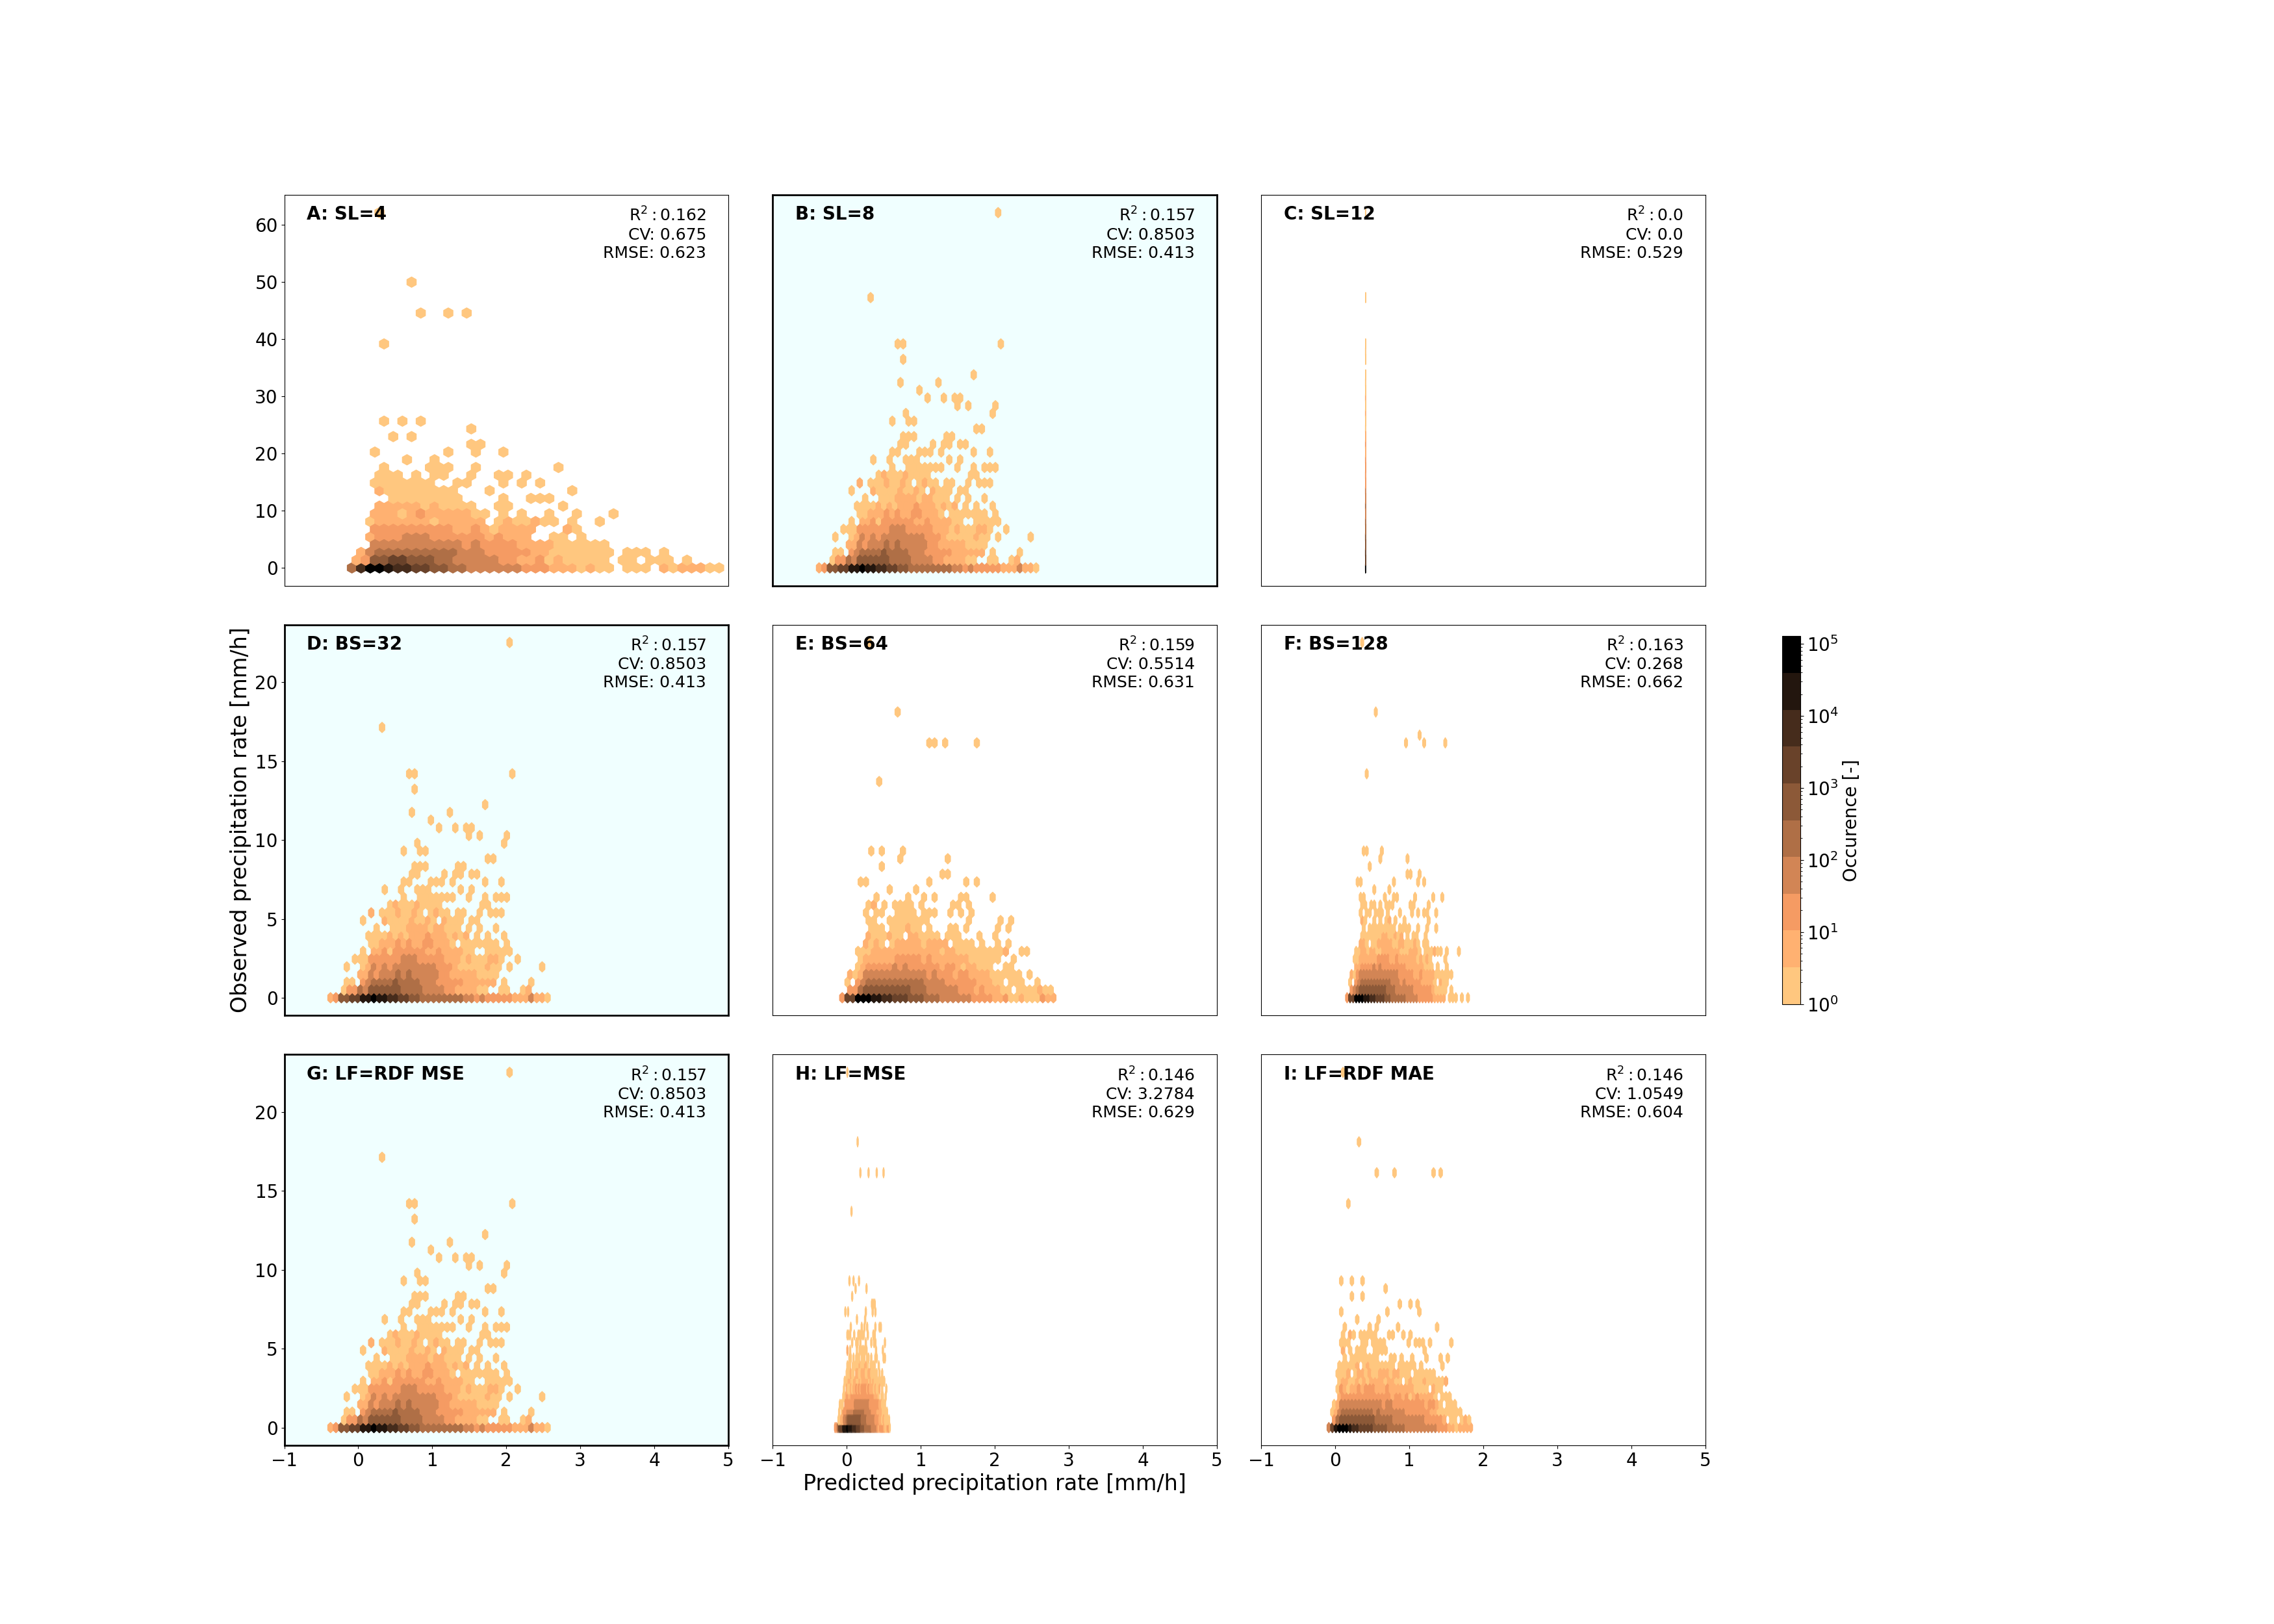
\includegraphics[width=25cm]{ex_seq_len}
		\vspace*{-1.5cm}
		\caption{Predicted versus observed precipitation rates for three varying hyperparameters: Sequence length (SL, plots ABC), Batch Size (BS, plots DEF) and Loss Function (LF, plots GHI). The lightblue black-outlined plots B, D and G indicate the default runs, where the default value of the specific hyperparameters are used.}
		\label{fig: seqlen}
	\end{figure*}

	\subsection*{Non-automated hyperparameter tuning}
	The impact of using a different sequence length, batch size or loss function is depicted in Figure~\ref{fig: seqlen}. These three hyperparameters were not automatically tuned. There is hardly any influence of the sequence length (Figure~\ref{fig: seqlen} ABC) on the predictions of the model. The observed variation between the runs stems from the random initialization of each run. Although there is some spread in the R\textsuperscript{2} values, it does not significantly improve the predictions. 
	
	The impact of the batch size (Figure~\ref{fig: seqlen} DEF) is equally difficult to describe, as there is little spread in the different results. One would expect a smaller batch size to perform better. The batch size of 32 has been found to generally yield the best results \cite{Bengio2012}, but that relation is not visible in these results, as the batch size of 64 and 128 are roughly performing equally well. The relation between learning rate and batch size is not investigated in this study and could be analyzed more thoroughly. This however is assumed to not be the major issue that causes the effect of the batch size to be virtually invisible. 
	
	The effect of the chosen loss function on the final results is minimal as well. Based on theory, the RDF MSE is expected to better steer towards higher values instead of constantly predicting a low average value. However, this is not entirely visible when comparing the runs with and without an RDF. The MAE is included to visualize the impact of the choice of loss function in general. There is hardly a difference visible between MAE and MSE, indicated by an almost identical R\textsuperscript{2} of [INSERT R2s HERE]. Although the loss function should be able to have quite an impact on the results, as it can be used to steer the model in a certain direction, this modelling effort has not shown anything of that impact. Based on these results, we cannot conclude that the loss function has a large influence on the results.

	\begin{figure}
		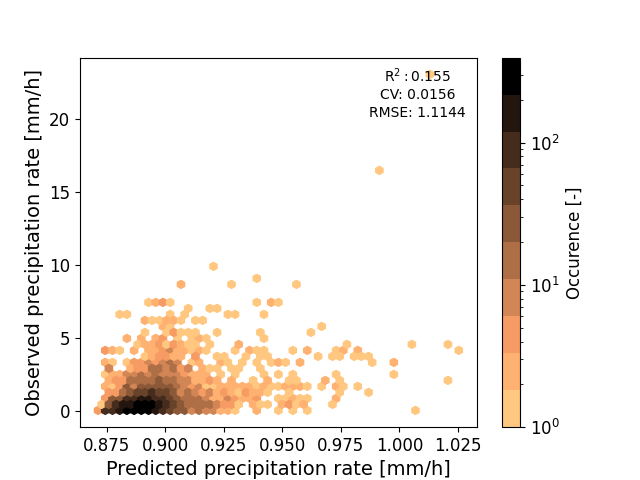
\includegraphics[width=\columnwidth]{scatter_onlyRain_final}
		\caption{Predicted versus observed precipitation with only wet samples included}
		\label{fig: onlyrain scatter}
	\end{figure}
	
	\subsection*{Wet samples only}
	Figure~\ref{fig: onlyrain scatter} shows the predicted precipitation when only wet samples are included. Although the predicted range is still smaller than the observed range in precipitation rates, the R\textsuperscript{2} indicates a slightly higher correlation between the two. Visually, there is more direction in the scatter compared to Figure~\ref{fig: scatter statistics}. Only including the wet samples improves the model, but the improvement is minor. Where the original model run had one specific precipitation rate that was preferred over all others, only including the wet samples leads to a wider spread in predicted values. The wet sample run does yield a better correlation, a slightly wider range and more direction in the scatter, but the results are still unsatisfactory and not suitable for operational use. 
	
	
	%%%%%%%%%%%%%%%%%%%%%%%%%
	%%%% DISCUSSION %%%%%%%%%
	%%%%%%%%%%%%%%%%%%%%%%%%%
	
	\chapter{Discussion} \label{ch: discussion}
	The discussion of this research is split up in two parts. The first parts deals with the more general assumptions and choices that have been made in this modelling effort and their implications, consequences and impacts, supported by previous studies. The second part, the outlook, deals with the poor outcomes of the tested deep learnings models for processing raw CML data for rainfall estimations. This part describes what could be included in future similar modeling efforts to improve the results of such an analysis.  
	
	Due to inefficient computational resources and various random errors throughout this study, the described methodology and approach has been applied to a depricated dataset. The original intent of using all links is still described and discussed in this section. Smaller try-out model runs on the complete dataset of all links indicated no significant difference in results between the depricated 10-link dataset and the full dataset. Therefore, the discussion that follows is still constructed like the full dataset is used, as the results are expected to be similar. 
	
	\section{Assumptions and choices}
	\subsection{Data splitting} \label{sec: discussion datasplitting}
	The chosen years are not identical in their precipitation distributions. The year 2011 was somewhat drier than average, with a particularly dry spring. 2012 was slightly wetter than average, with above average precipitation in the first and last months of the year. Finally, 2013 had a dry winter with some snow, yielding a yearly average precipitation considerably lower than average. \cite{KNMI2022}  
	This inconsistency in precipitation over the years violates the IID assumption that underpins the data split. It highlights the tradeoff that has been made in creating this split. Ideally, all datasets would have an equal identical precipitation distribution. However, wherever two datasets meet in time, there is a chance of information leaking from one dataset to the other. If the years would have been reshuffled to create a more identically distributed split, there would have been more information leaking from one set to the other and the independence of the datasets would have been at stake. Therefore, this split by full years was still preferred, to minimize information leakage. For the test set, half a year is taken due to limitations in data availability. As the validation set is only used to judge the final model, and not to update the model anymore, this dataset can be smaller as for example in \citeA{Pudashine2020}.
	
	Due to the aforementioned reasons, the data is not perfectly IID. Apart from the more abstract discussion whether the IID principle is ever really attainable (as there are always some long term dependencies in data; \citeA{Hampel1998}), the impact of not conforming to IID has been discussed before. Several studies have dealt with data that is not IID. \shortciteA{Lin2016} proposed a method where the non-IID data is further split up in small groups that can be assumed to be IID. The loss per group is determined and the maximum average loss per group was taken as a loss function. \shortciteA{Xu2019} suggested a numerical algorithm to solve this method for non-linear problems.
	
	Although the data is not conforming to IID, during this study we deemed it non necessary to implement a specific algorithm suitable for non-IID data. Both training and validation data include all 4 seasons, have a full year span (~80 million data points) and have not been filtered on any sort of events. When the model would be evaluated with a completely new independent dataset, this dataset could also include the natural variability that is present in these datasets. As the sets are long enough, the effect of not perfectly IID data is assumed to not have a major influence on the final results. This assumption is supported by the results presented in Figure~\ref{fig: onlyrain scatter}. Studies that used similar data before used a similar split of the data, assuming that this split guarantees the data to be sufficiently IID \cite{Diba2021,Pudashine2020}. Other follow-up studies could use a bootstrapping method where the datasets are shuffled (e.g. validating on 2012) to assess the sensitivity of the model to the chosen data split. 
	

	
	
	\subsection{Optimal hyperparameter combination} \label{sec: Equifinality}
	In selecting hyperparameters to tune automatically, a few choices have been made. Their ranges have been determined based on previous studies and conventions, but that does exclude some values. In tuning hyperparameters, \citeA{Breuel2015} showed that the optimal combination of hyperparameters is not a very narrow space. Every hyperparameter has its own regions in which the final results are comparable. In tuning these hyperparameters, it is more about roughly searching the whole hyperparameter space than to include every single combination. There might even be multiple hyperparameter combinations that all result in the same best result. Figure~\ref{fig: loss epochs} shows that most of the combinations are relatively close and their final outcome is mainly determined by the random initialization. 
	
	This concept of equifinality is not new in physically-based and conceptual hydrological studies \cite<e.g.>{Schulz1999,Bardossy2008} and has been discussed in a data-driven modelling context as well \shortcite{Yoon2011,Shamseldin2002}. One method to deal with this equifinality concept in models is to make use of the Generalised Likelihood Uncertainty Estimation \cite<GLUE,>{Beven2001}. This methodology is based on creating an ensemble prediction by running different simulations with different parameter values and assess their likelihood. In this study, the GLUE methodology has not been used. Part of the research is to investigate the sensitivity of the model results to any changes in the hyperparameters. The different runs serve the purpose of covering a reasonably large set of hyperparameter configurations to indicate whether a further analysis into hyperparameter sensitivity would be necessary. The results in this study are difficult to interpret, as they do not resemble a decent fit in any way, shape or form (R\textsuperscript{2} = INSERT R2 VALUE HERE). There is variation between model runs with different hyperparameter configurations, but just because they are better does not mean that they are good to any extent. A concrete recommendation on whether applying the GLUE methodology in future studies is therefore difficult to pose. Supposed that the results from the first try would be more satisfactory, a GLUE sensitivity analysis of the hyperparameters in the model would be useful to better quantify the impact certain hyperparameters have. 
	
	
	\subsection{Model architecture} \label{sec: no results} 
	This study uses an LSTM model as main architecture. Based on this architecture, tuning to optimize hyperparameters and other analyses are performed. However, although LSTM is a commonly used method in time series prediction and sequential data, it is not the only suitable model out there. \citeA{Polz2020} used a 1D-convolutional neural network, \citeA{DordevicYear} proposed a multi-layer perceptron artificial neural network and \citeA{Habi2019} used both LSTM and Gated Recurrent Unit models, although the latter two are quite alike. This spread highlights two things: 1) neural networks are versatile and come in different shapes and sizes and 2) multiple architectures can lead to similarly good results, which touches upon the concept of equifinality as discussed before. The use of LSTMs in this study is not assumed to be the key factor that causes the poor results. As different model architectures lead to similar results, the influence of the selected architecture is deemded quite small (given that the selected architecture is theoretically suitable for estimating precipitation sequences).
	
	\subsection{Mid-link approach} \label{sec: middle link}
	To obtain the precipitation rates corresponding to every CML, this study uses a mid-link approach, where the middle of the link is taken as the representative location for the gauge-adjusted radar product. This approach negates one of the advantages of using CML signals to retrieve rainfall rates, which is the opportunity to report a path-averaged rainfall rate \cite{Pudashine2020}. The assumption in this study is that as the majority of the links are quite short (<3-4 km, see figure~\ref{fig: CML validation} b), having one middle reference point is sufficient. This assumption is in line with amongst others \citeA{Pudashine2020} and \citeA{Diba2021}.
	However, a more robust approach is to use a weighted average of all radar cells on the link path. This method has been succesfully studied and implemented by \citeA{Leijnse2007} and \citeA{Polz2020}. The main advantage of this method compared to the mid-link approach is that spatially highly variable precipitation can be attributed for.Moreover, averaging over multiple pixels causes less sampling noise. The longer the link, the larger the possible missed events can be. These highly variable precipitation events, however, do not occur often in the years that are studied \cite{KNMI2022}. Switching between the mid-link approach and the weighted average method would imply a complete restructuring of the data and is out of the scope of this research. Although the results are expected to improve when the latter method is chosen, is it difficult to quantify the degree to which as the model used in this study is not able to pick up any signal-precipitation relation at all. No comparative studies between the two methods have been performed. The mid-link approach is easier and faster but the simplification does come at the cost of accuracy for small-scale events.  
	
	\subsection{Local minima} \label{sec: local minima}
	The observed behaviour of the model in this study, where it is unable to find the right set of weights and biases to fit the received signal to the precipitation, is linked to local minima in the modelling landscape. In looking for the optimal weights and biases, the ADAM optimizer efficiently looks for the steepest gradient in any direction and steers the model parameters towards that direction. There seem to be a lot of local minima present in this model which tend to result in predicting a single constant for all samples. Finding a local minimum instead of a global minimum is a more common problem in complex, multi-parameter models and calibration of such models has been studied extensively \cite{Duan1992,Arsenault2014}. A neural network is essentially a model with many parameters. A 4-layer LSTM with a sequence length of 8 is dealing with 160 weights at the same time. Although the ADAM optimizer is widely used throughout different applications of neural networks, there do exist different methods and optimizers that claim to more effectively find the global minimum when calibrating neural networks \cite{Bianchini1994}. 
	
	More convential ways to make sure the calibration procedure finds the global minimum are to widen the search space to the entire domain and to increase the number of calibration runs that are executed, to increase the chances of finding this global minimum. Both of these ways have been applied to this model as well, without succes. The number of tuning runs was deemed insufficient. An algorithm like the one suggested by \citeA{Bianchini1994} could improve the results, although the question should be asked whether the problem of these local minima is the main problem occurring in this modelling effort. 
	
	\section{Outlook}
	This study has shown that a multi-layer LSTM is not capable of estimating rainfall rates with raw CML data only. There is hardly any relation found between the CML signal and the observed precipitation. At the start of this study, we hypothesized that an LSTM should be capable of this, as neural networks and specifically LSTMs excel at finding those relationships in sequential data. The studies that are cited throughout this thesis show that it is possible to use neural networks for this CML application, albeit with some minor changes to the methodology. The methodology that I studied in this thesis, where I completely replaced the 4-step RAINLINK process by one all-encompassing neural network with some minor adjustments to aid the model, has not proven to work in its current shape. Below, there are 5 improvements to the current modelling effort that, based on previous work, should help in getting the final model in the direction that we envisioned at the start. 
	
	\subsection*{Nearby link approach} \label{sec: nearby link}
	In RAINLINK, there is a thorough wet-dry classification which uses the nearby link approach \cite{Overeem2011}. This approach is based on the idea that if it rains in one link, links within a certain radius should experience rain as well. This wet-dry classification prevents other clutter that could distort the signal, like birds, to be included in the data. By including such a wet-dry classification and splitting before training, \citeA{Diba2021} and \citeA{Pudashine2020} have found more credible results.
	Not all studies include this nearby link approach, but most do include some sort of a wet-dry classfication to aid the model. The results in this study have shown that only including wet samples help the prediction a little bit. In future similar modelling efforts, a wet-dry classification of some sort should more explicitly be included. This can either be done before running the model, or by passing nearby links through the model as well, to let the model learn the relation between the links. This requires a slightly different modelling set-up and a different datastructure, but would possibly lead to improved results. Based on the coordinates of each link, extra static data could be included that indicates which links are close to each other. As not all links have a nearby link within a short radius, the model needs to be able to deal with different input sizes and shapes.
	
	\subsection*{Baseline estimation} \label{sec: baseline}
	By subtracting the median of each link per dataset from the signal, a very crude baseline estimation has been performed in this study. RAINLINK uses a 24-h median to calculate the baseline method, and other studies \cite{Habi2019} have used a similar method as well. The difference between the two methods is small and would probably not have a major influence on the final results. The additional scaling that is applied (dividing by the standard deviation) is not expected to have a major influence on the outcome of the model. In future similar modelling efforts, a more rigorous baseline estimation should be included. This can either be done in the data preprocessing phase, or, similar to in section~\ref{sec: nearby link}, a longer timeseries can be added to the model in order to learn what the baseline is for a specific signal. It should be noted that the former option is preferred, as adding more data to the model requires the model to take longer to learn, to update more parameters and ultimately makes it more difficult for a neural network to fully grasp the underlying relationships in the data. 
	
	\subsection*{Split up the steps in multiple models}
	All steps of the RAINLINK algorithm have been included in one single model in this study. An alternative would be, similar to for example \citeA{Habi2019}, to create a separate deep learning model for the different steps in the RAINLINK algorithm. Feeding the data through a classification network that performs a wet-dry classification, or a separate multilayer perceptron model to calculate the wet antenna attenuation would allow to tailor the specific models to the specific steps. Having one big model has proven to be inefficient at the task of estimating precipitation. It is not possible to capture the whole RAINLINK methodology in one single model.
	
	\subsection*{Include static metadata}
	Not all studies on using neural networks for estimating precipitation from CML data include multiple links. Dealing with multiple links gives the modeller the opportunity to tune the model to more data, but it does come with a few extra challenges. The static metadata (see Section~\ref{sec: CML data} and~\ref{sec: discussion datasplitting}) differs per link and influences the baseline of the signal and how sensitive the signal is to rain. It is for those two reasons that \citeA{Habi2019} included a separate model where the static metadata per link (frequency, link path length and tower height) was added. The downside of including this data is that it becomes more difficult to envision what is going on inside the model: it strengthens the black-box character that neural networks are susceptible to. This is the reason that these kind of data were not explicitly included in this study. Efforts have been made to include distance and frequency as predictors using the current architecture, but these have not lead to any major improvements. In future similar modelling efforts, a separate part on static metadata could help the model in differentiating between the different links and therefore improve the precipitation estimation. 
	
	\subsection*{Bottom-up approach}
	This research was conducted along an optimistic top-down modelling approach: we started with modelling the whole 4-step methodology and when the results were unsatisfactory, we tried different small changes to improve the results. We have not been able to explore the boundaries of the model using this approach, as the final efforts still yielded incorrect results. These boundaries can show us the power of such deep learning models and are thus interesting to study. For a future similar modelling effort, we suggest a bottom-up, more pessimistic approach. By starting with a known and working model and gradually making changes towards a fully deep-learning model, these boundaries can be explored in a differently structured way. If one aspect is replaced by a deep learning effort at a time, the exact threshold at which the model does not function properly anymore can be determined.  
	
	

	%%%%%%%%%%%%
	% CONCLUSION
	%%%%%%%%%%%%
	
	\chapter{Conclusion} \label{ch: conclusion}
	This study focused on using one all-encompassing neural network to replace all 4 steps in the RAINLINK algorithm to estimate precipitation using Commercial Microwave Links (CML). By taking inspiration from different previous studies, a modelling effort has been made to link the received signal levels from CMLs to precipitation rate. Signal levels at 15-min resolution for ~2500 links throughout a time period of 2,5 years have been used as input data to a self-learning Long Short Term Memory (LSTM) model. Different hyperparameter configurations of this model have been explored both automatically and manually. Different model architectures and preprocessing of the data (e.g. only using wet samples) have been used as well to assess the sensitivity of the constructed model to these factors. Based on this study, it can be concluded that the approach taken does not yield satisfactory results and does not yield a model able to correctly estimate precipitation rates based on these received signal levels.
	
	The sensitivity of the model to several hyperparameters has been tested, in order to see what their influence on the final result would be. None of these hyperparameters have shown to have a significant influence on the prediction of the model, mainly because the model is not able to pick up any signal. None of the explored hyperparameter configurations showed to improve the model significantly. 
	
	It is thus not possible to cover all 4 steps of the RAINLINK algorithm using one all-encompassing LSTM neural network. The hyperparameters in this study have had no influence on this result. Future attempts at similar modelling efforts should include a more thorough wet-dry classification (if possible a nearby-link approach), and split up the model in separate models for the different tasks in the RAINLINK methodology.  
	
	%%%%%%%%%%%%%%%%%%%%%%%%%%%%%%%%%
	% ACKNOWLEDGEMENTS
	%%%%%%%%%%%%%%%%%%%%%%%%%%%%%%%%%
	


	\chapter*{Acknowledgements}\vspace{-6mm}       % the * prevents numbering of this section
	\addcontentsline{toc}{chapter}{Acknowledgements}   % to get acknowledgements in table of contents
	\markboth{Acknowledgements} {}
	I would like to thank Ralph Koppelaar and Ronald Kloeg from T-Mobile and Aart Overeem from KNMI for supplying the CML data over the 2,5 years of interest to this study. I would like to thank Daniel Teixeira Soares Tolomei for thinking along with the programming aspect of this study and Andrea Pagani for his interesting thoughts on neural networks and transfer learning. Finally, a big thanks to Kirien Whan, who helped supervising this thesis purely out of interest for the topic.

	%%%%%%%%%%%%%%%%%%%%%%%%%%%%%%%%%
	% BIBLIOGRAPHY
	%%%%%%%%%%%%%%%%%%%%%%%%%%%%%%%%%
	%\renewcommand\bibname{Bibliography}
	\markboth{Bibliography}{Bibliography}
	
	\bibliographystyle{myapacite}
	\bibliography{Thesis_Ludo}
	
	% to add items to the bibliography:
	% option 1. open "references_thesis.bib" in JabRef (free downloadable), enter more papers
	% option 2. open "references_thesis.bib" in NotePad, go to Google Scholar, find paper, click "cite", click "import into BiBTeX", copy text into NotePad
	
	
	%%%%%%%%%%%%%%%%%%%%%%%%%%%%%%%%%
	% APPENDIX
	%%%%%%%%%%%%%%%%%%%%%%%%%%%%%%%%%
	
	%\appendix
	%\chapter{Additional figures}
	
	
	%%%%%%%%%%%%%%%%%%%%%%%%%%%%%%%%%
	% END
	%%%%%%%%%%%%%%%%%%%%%%%%%%%%%%%%%
	
	
\end{document}